<<<<<<< HEAD
\section{Ejercicio 2: Comparaci\'on de compuertas discretas con tecnolog\'ia TTL y CMOS}
Se plantea estudiar la compatibilidad de compuertas de tecnología TTL (a base de transistores BJT) con CMOS (transistores MOSFET), enfocando la problemática desde el 
estudio de sus características de márgen de ruido, y haciendo también mención al fanout. 
Se abordará este análisis mediante el estudio de caso de los integrados 74HC02, 74HCT02 y 74LS02, los cuales contienen 4 compuertas NOR cada uno, implementados mediante 
distintas tecnologías.



\subsection{Marco teórico}
Las letras LS en 74LS02 refieren "Low-power Schottky", una tecnología del tipo TTL que alcanza mejores rendimientos y velocidad gracias a la implementación de 
transistores Schottky, los cuales difieren de los clásicos BJT únicamente en el agregado de un diodo Schottky entre sus terminales Base y Colector.
Por otro lado, HC y HCT refieren a "High-speed CMOS", distinguiéndose HCT por ser compatible con las tecnologías TTL.

\begin{figure}[H]
    \centering
    \begin{tabular}{c c}
        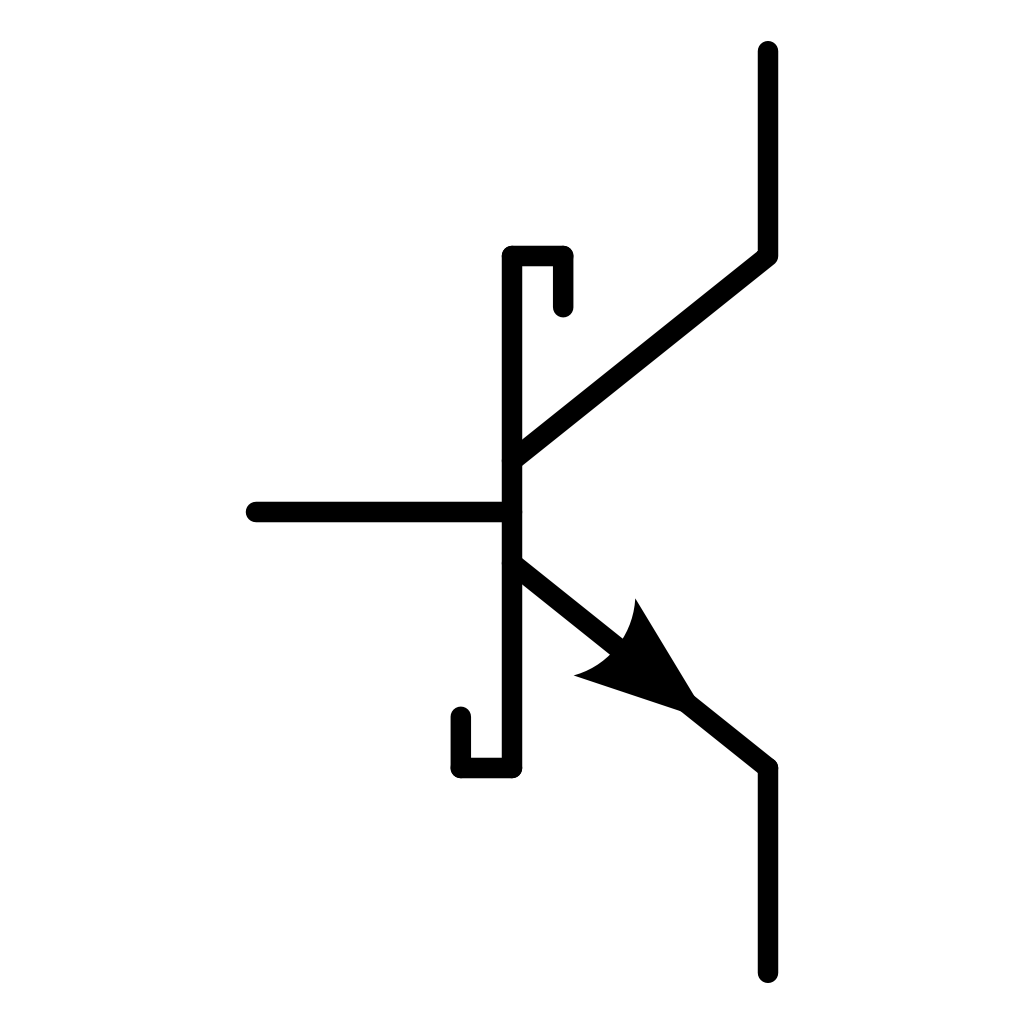
\includegraphics[width=0.1\textwidth]{../EJ2/Recursos/schottky_transistor_symbol} &
        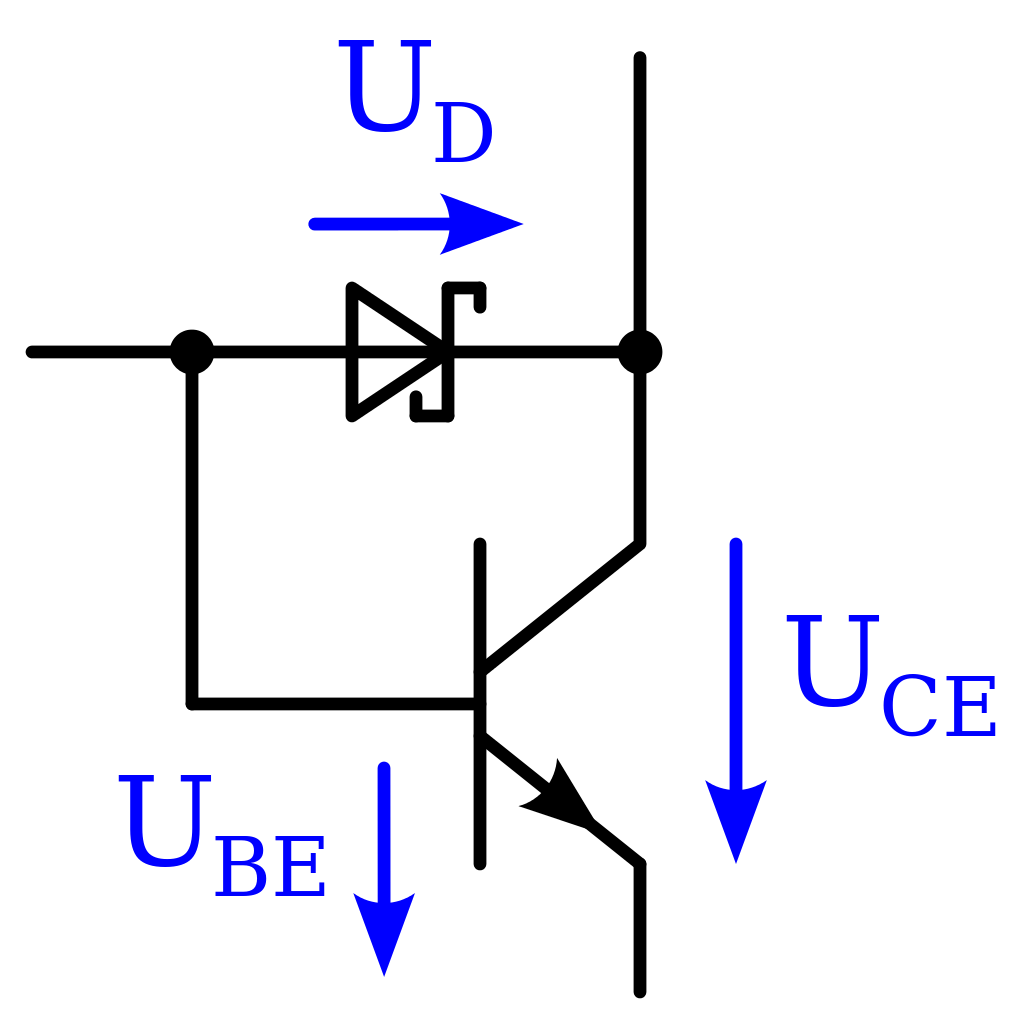
\includegraphics[width=0.1\textwidth]{../EJ2/Recursos/schottky_transistor_circuit}
    \end{tabular}
    \caption{Símbolo y circuito de transistor Schottky.}
    \label{fig:schottky_transistor_symbol_and_circuit_ex5}
\end{figure}

Tal y como fue mencionado en el inicio de esta sección, en este trabajo se estudiará la compatibilidad entre las tecnologías a través de sus márgenes de ruido.
Esto significa que, en términos de interconexión, una compuerta solo será compatible con otra de otra tecnología, si el rango de valores de salida de la primera está 
incluido en el rango de entrada de la segunda. \\
En las figuras \ref{fig:compatible_v_non_compatible_ex5} y \ref{fig:compatible_v_non_compatible_2_ex5} pueden apreciarse los casos que pueden presentarse que significarán la compatibilidad o no entre las compuertas.
De ellos se extrae que las compuertas serán compatibles solo en el caso en que $V_{OH} \geq V_{IH}$ y $V_{OL} \leq V_{IL}$.

\begin{figure}[H]
    \centering
    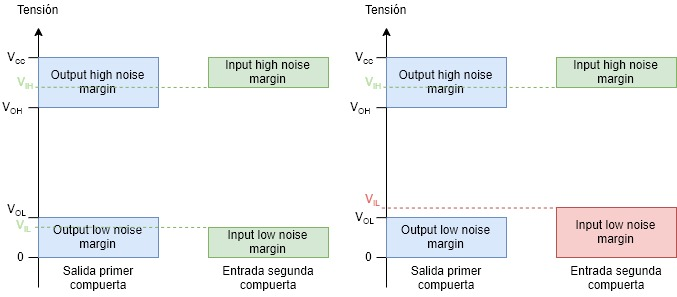
\includegraphics[width=0.9\textwidth]{../EJ2/Recursos/compatible_gates}
    \caption{Compatibilidad de compuertas.}
    \label{fig:compatible_v_non_compatible_ex5}
\end{figure}

\begin{figure}[H]
    \centering
    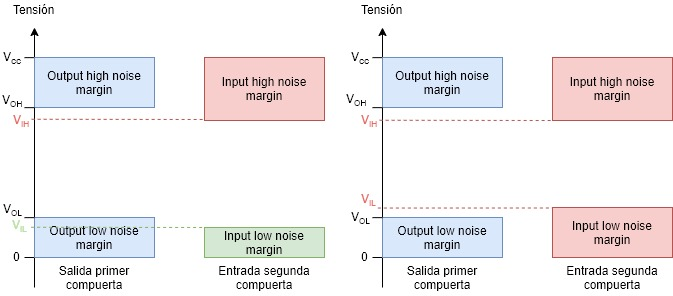
\includegraphics[width=0.9\textwidth]{../EJ2/Recursos/incompatible_gates}
    \caption{Compatibilidad de compuertas.}
    \label{fig:compatible_v_non_compatible_2_ex5}
\end{figure}

Con respecto al fanout, el mismo es una limitación para la cantidad de compuertas que se pueden colocar a la salida de otra, que viene dada por las corrientes de entrada 
y salida, respectivamente.

\begin{equation}
    fanout = min\left(\frac{I_{OH}}{I_{IH}} ; \frac{I_{OL}}{I_{IL}}\right)
\end{equation}



\subsection{Análisis mediante hojas de datos}
Se estudia la compatibilidad de la interconexión de las compuertas mediante la observación de las hojas de datos de los integrados 
74HC02\footnote{http://pdf.datasheetcatalog.com/datasheet/NXP\_Semiconductors/74HC\_HCT02.pdf}, 74HCT02\footnote{http://pdf.datasheetcatalog.com/datasheet/NXP\_Semiconductors/74HC\_HCT02.pdf} y 74LS02\footnote{http://www.sycelectronica.com.ar/semiconductores/74LS02.pdf},
y se exponen los datos utilizados en la tabla \ref{table:parameters_datasheet_ex5}.
Cabe mencionar que las condiciones de prueba de estos parámetros no son las mismas para las compuertas de tecnología CMOS que para las de TTL, de modo que se decide tomar 
el caso más desfavorable para cada una de las comparaciones.
En todos los casos, este terminó siendo que para las compuertas HC y HCT, la alimentación es de $4,5 V$, mientras que para las LS es de $5 V$.

\begin{table}[H]
    \begin{tabular}{ccccccccc}
    \textbf{Integrado} & \textbf{$V_{OH}$} & \textbf{$V_{OL}$} & \textbf{$V_{IH}$} & \textbf{$V_{IL}$} & \textbf{$I_{OH}$} & \textbf{$I_{OL}$} & \textbf{$I_{IH}$} & \textbf{$I_{IL}$} \\ \hline
    \textbf{74HC02}    & $4,4 V$           & $0,1 V$           & $3,15 V$          & $1,35 V$          & $\pm 25 mA$       & $\pm 25 mA$       & $\pm 0,1 \mu A$   & $\pm 0,1 \mu A$   \\
    \textbf{74HCT02}   & $4,4 V$           & $0,1 V$           & $2 V$             & $0,8 V$           & $\pm 25 mA$       & $\pm 25 mA$       & $\pm 0,1 \mu A$   & $\pm 0,1 \mu A$   \\
    \textbf{74LS02}    & $2,7 V$           & $0,5 V$           & $2 V$             & $0,8 V$           & $-0,4 mA$         & $8 mA$            & $20 \mu A$        & $-0,4 mA$        
    \end{tabular}
    \caption{Parámetros de compatibilidad obtenidos de datasheet.}
    \label{table:parameters_datasheet_ex5}
\end{table}

Se desprende de los datos expuestos y de la teoría explicada en el marco teórico, que son compatibles las conexiones de una compuerta HC a LS, de una HCT a LS, y de una 
LS a una HCT, ya que en todos estos casos se cumple que $V_{OH} \geq V_{IH}$ y $V_{OL} \leq V_{IL}$.
También es este el caso entre HCT y HC, y viceversa, resultado que es de esperar ya que comparten el tipo de tecnología.
Sin embargo, no sucede esto al ir de una LS a una HC ya que para esta combinación $V_{OH} < V_{IH}$, quedando una zona de indeterminación entre los valores de tensión 
$2,7 V$ y $3,15 V$.
Esta incompatibilidad es lógicamente salvada al usar tecnología HCT, la cual está diseñada con el propósito de lograr la compatibilidad que carecen las compuertas HC 
entre tecnologías TTL y CMOS.\\
En lo que respecta al fanout, los resultados son los expuestos en la tabla \ref{table:fanout_results_ex5}
\begin{table}[H]
    \begin{tabular}{ccccccc}
    \textbf{Interconexión} & \textbf{HC a LS} & \textbf{LS a HC} & \textbf{HCT a LS} & \textbf{LS a HCT} & \textbf{HC a HCT} & \textbf{HCT a HC} \\ \hline
    \textbf{fanout}        & $62$             & $4000$           & $62$              & $4000$            & $250 \cdot 10^3$  & $250 \cdot 10^3$ 
    \end{tabular}
    \caption{Fanout para distintas conexiones.}
    \label{table:fanout_results_ex5}
\end{table}



\subsection{Resultados experimentales}
Para el caso donde las hojas de datos no aseguran el correcto funcionamiento de la interconexión de compuertas, es decir, de una LS a una HC, se procede a estudiar su 
respuesta de forma experimental.
Se alimenta una compuerta del 74LS02 utilizada como NOT (cortocircuitando sus dos entradas) con una función rampa de 0 a 5V, y a su salida se conecta una del 74HC02, 
también como NOT. 
Se miden las salidas de ambas y los resultados son los expuestos en las figuras \ref{fig:LS_L_v_HC_H_ex5} y \ref{fig:LS_H_v_HC_L_ex5}.\\
Luego se realiza el mismo procedimiento pero en el lugar del 74HC02 se coloca el 74HCT02, cuyos resultados son los de las figuras \ref{fig:LS_L_v_HCT_H_ex5} y \ref{fig:LS_H_v_HCT_L_ex5}.
Se esperan observar indeterminaciones para la primer interconexión, y que tales problemas se vean resueltos al cambiar la tecnología HC por HCT. 

\begin{figure}[H]
    \centering
    \begin{tabular}{c c}
        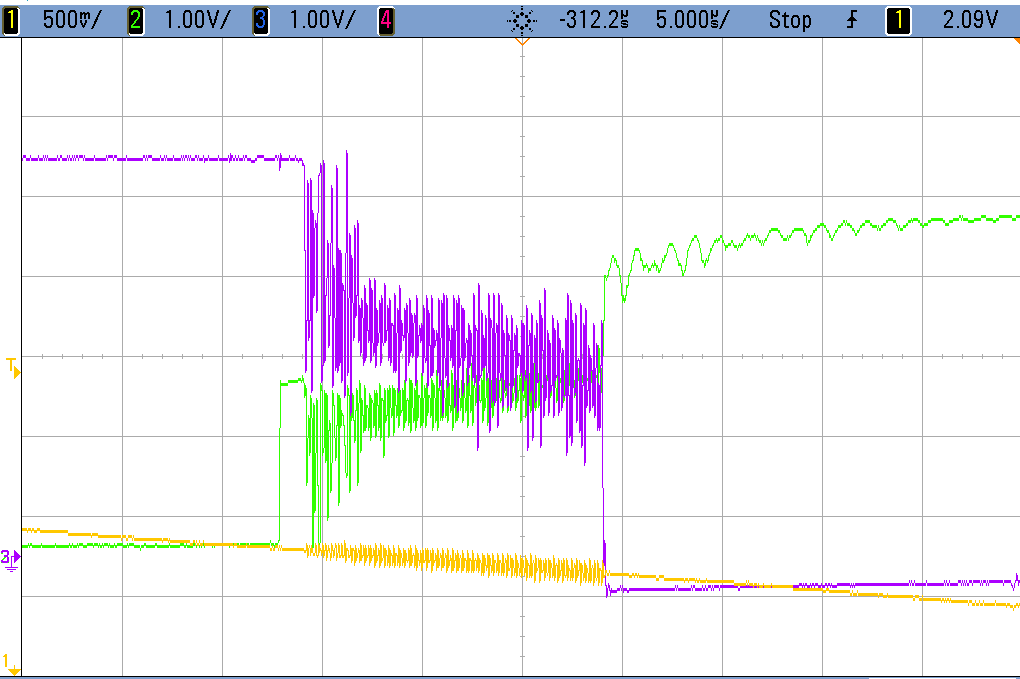
\includegraphics[width=0.5\textwidth]{../EJ2/Recursos/scope_32} &
        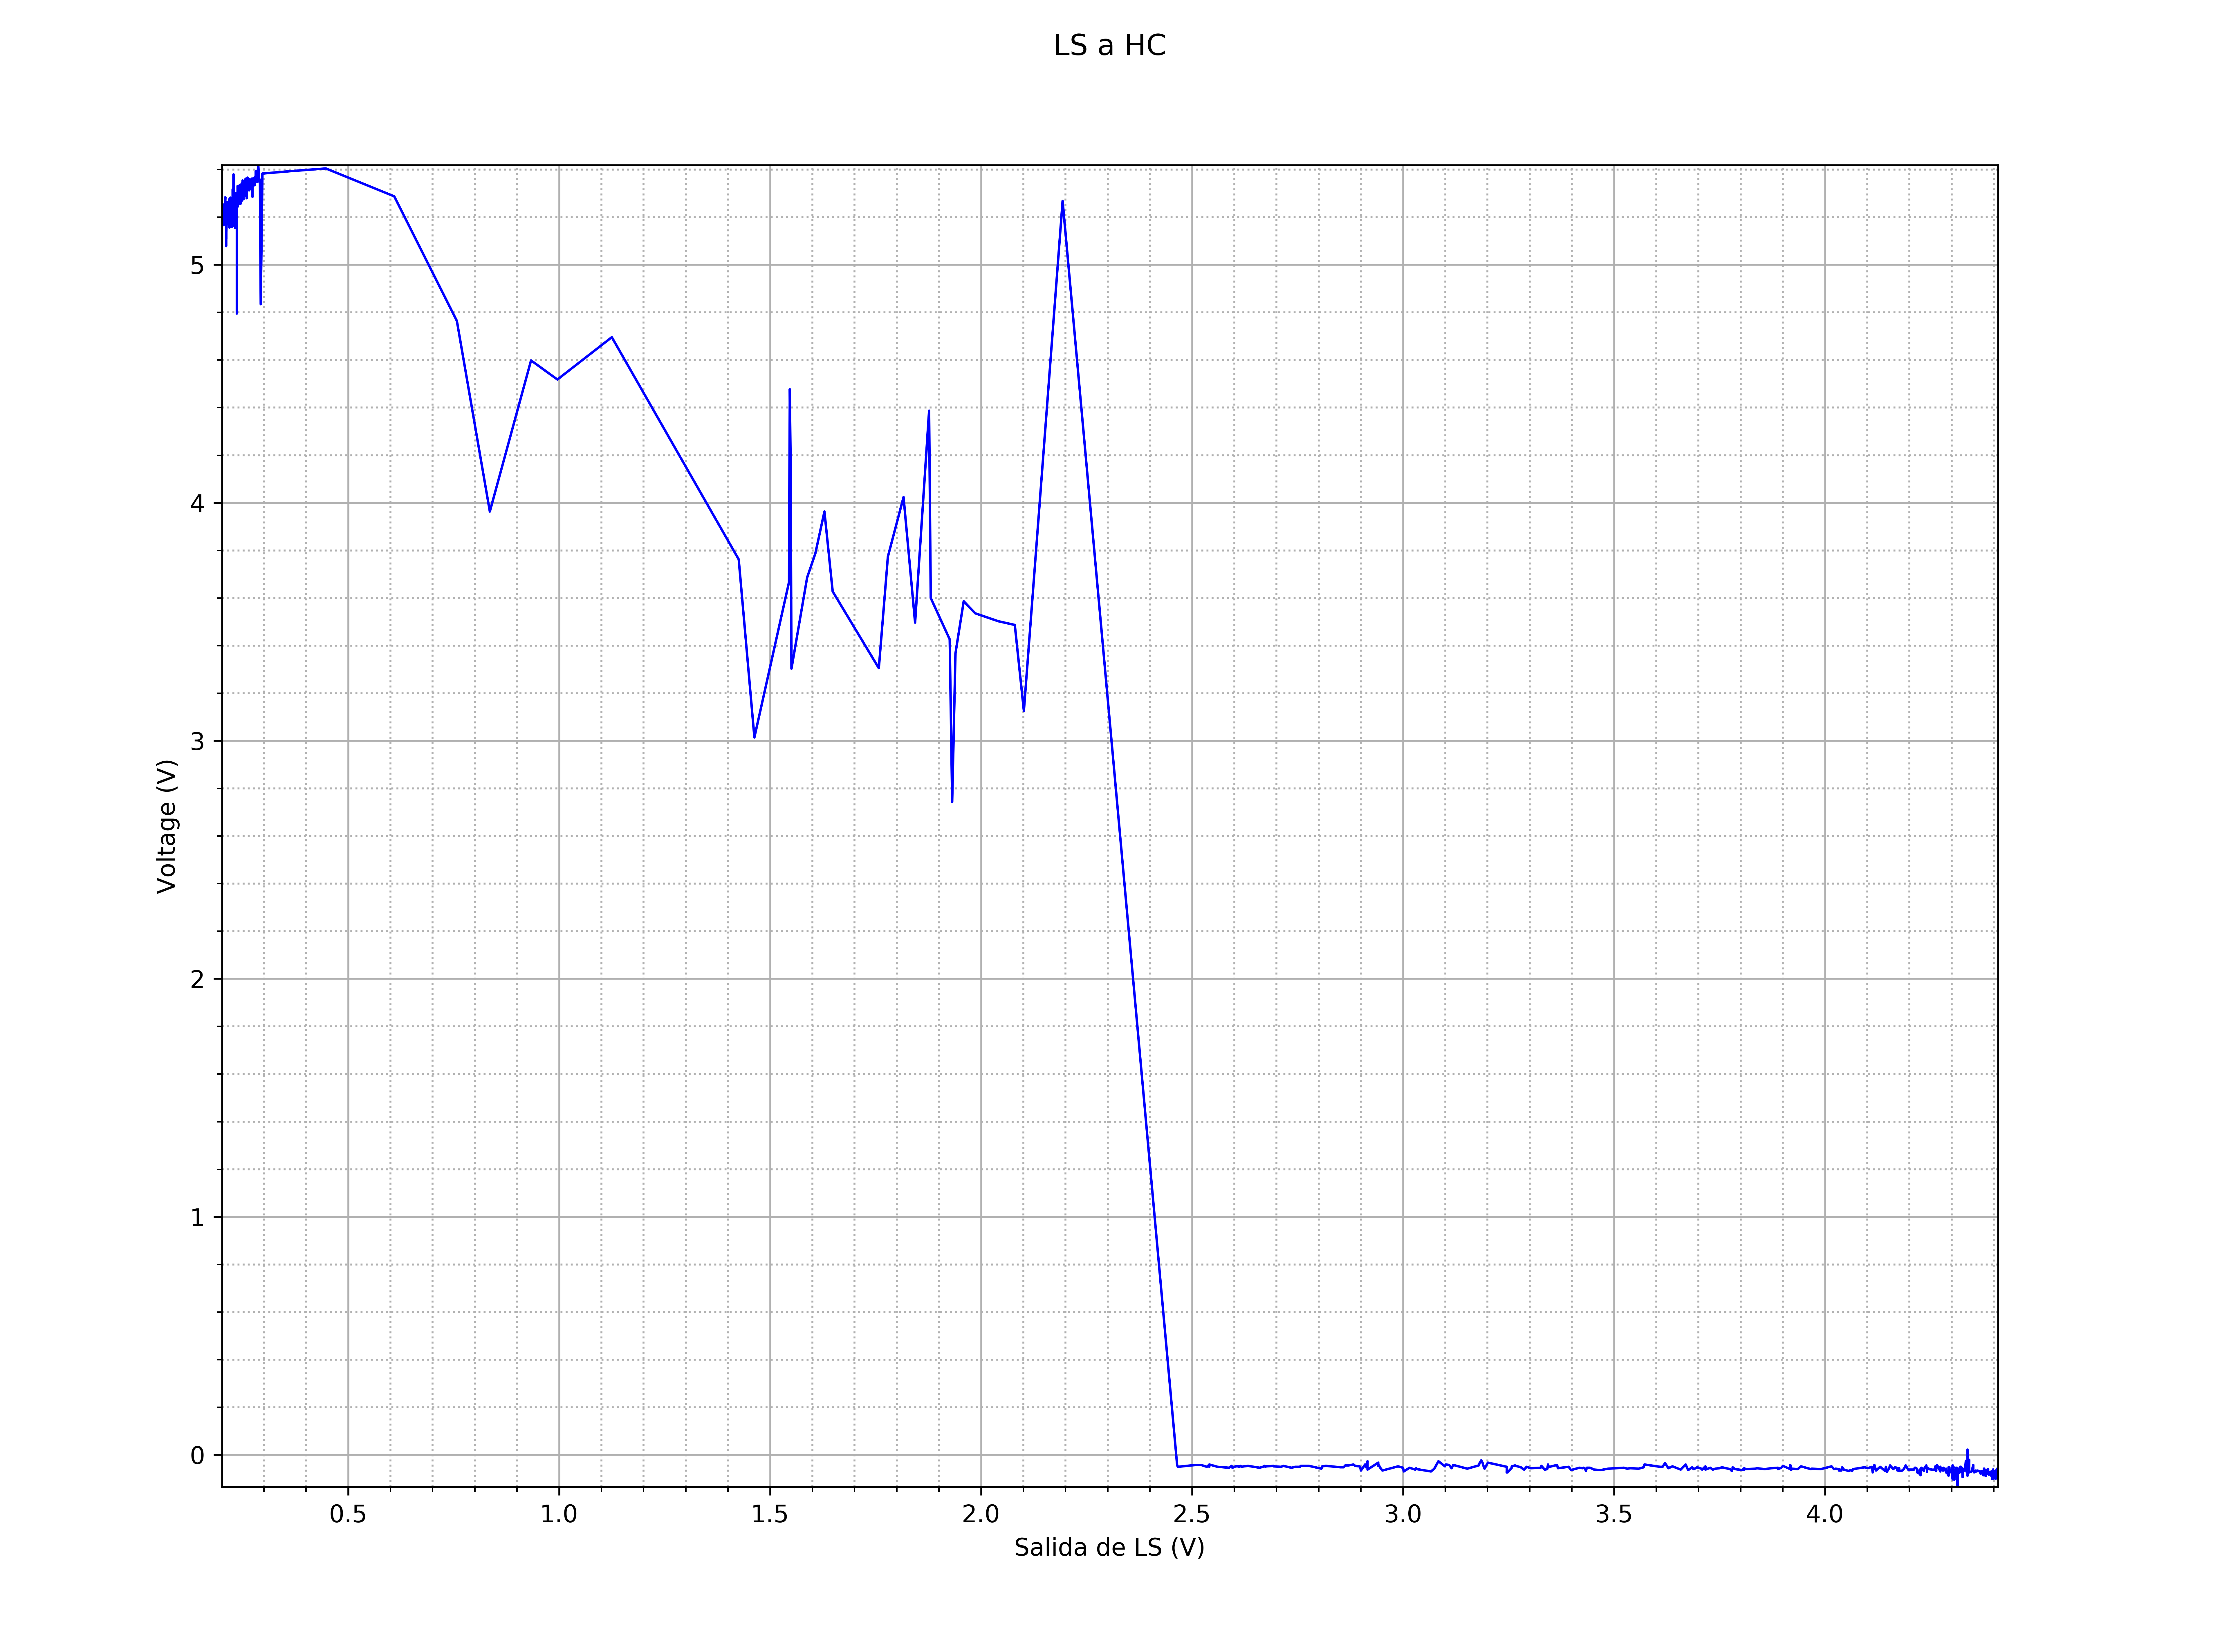
\includegraphics[width=0.5\textwidth]{../EJ2/Recursos/LS_L_v_HC_H}
    \end{tabular}
    \caption{LS a HC, con LS pasando de 0 a 1, y HC de 1 a 0.}
    \label{fig:LS_L_v_HC_H_ex5}
\end{figure}
\begin{figure}[H]
    \centering
    \begin{tabular}{c c}
        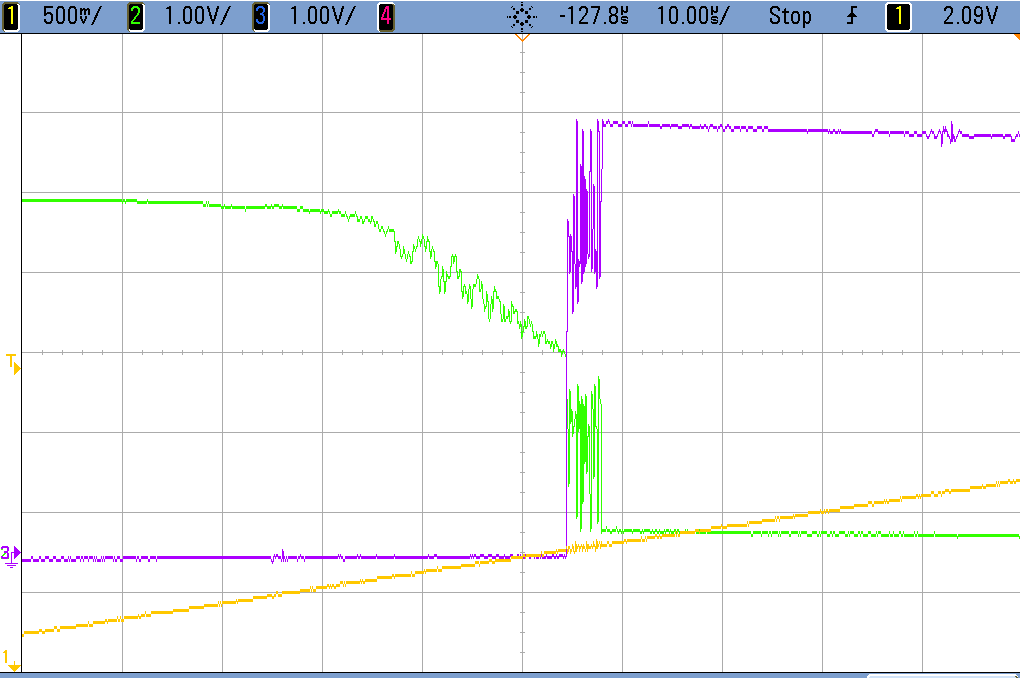
\includegraphics[width=0.5\textwidth]{../EJ2/Recursos/scope_29} &
        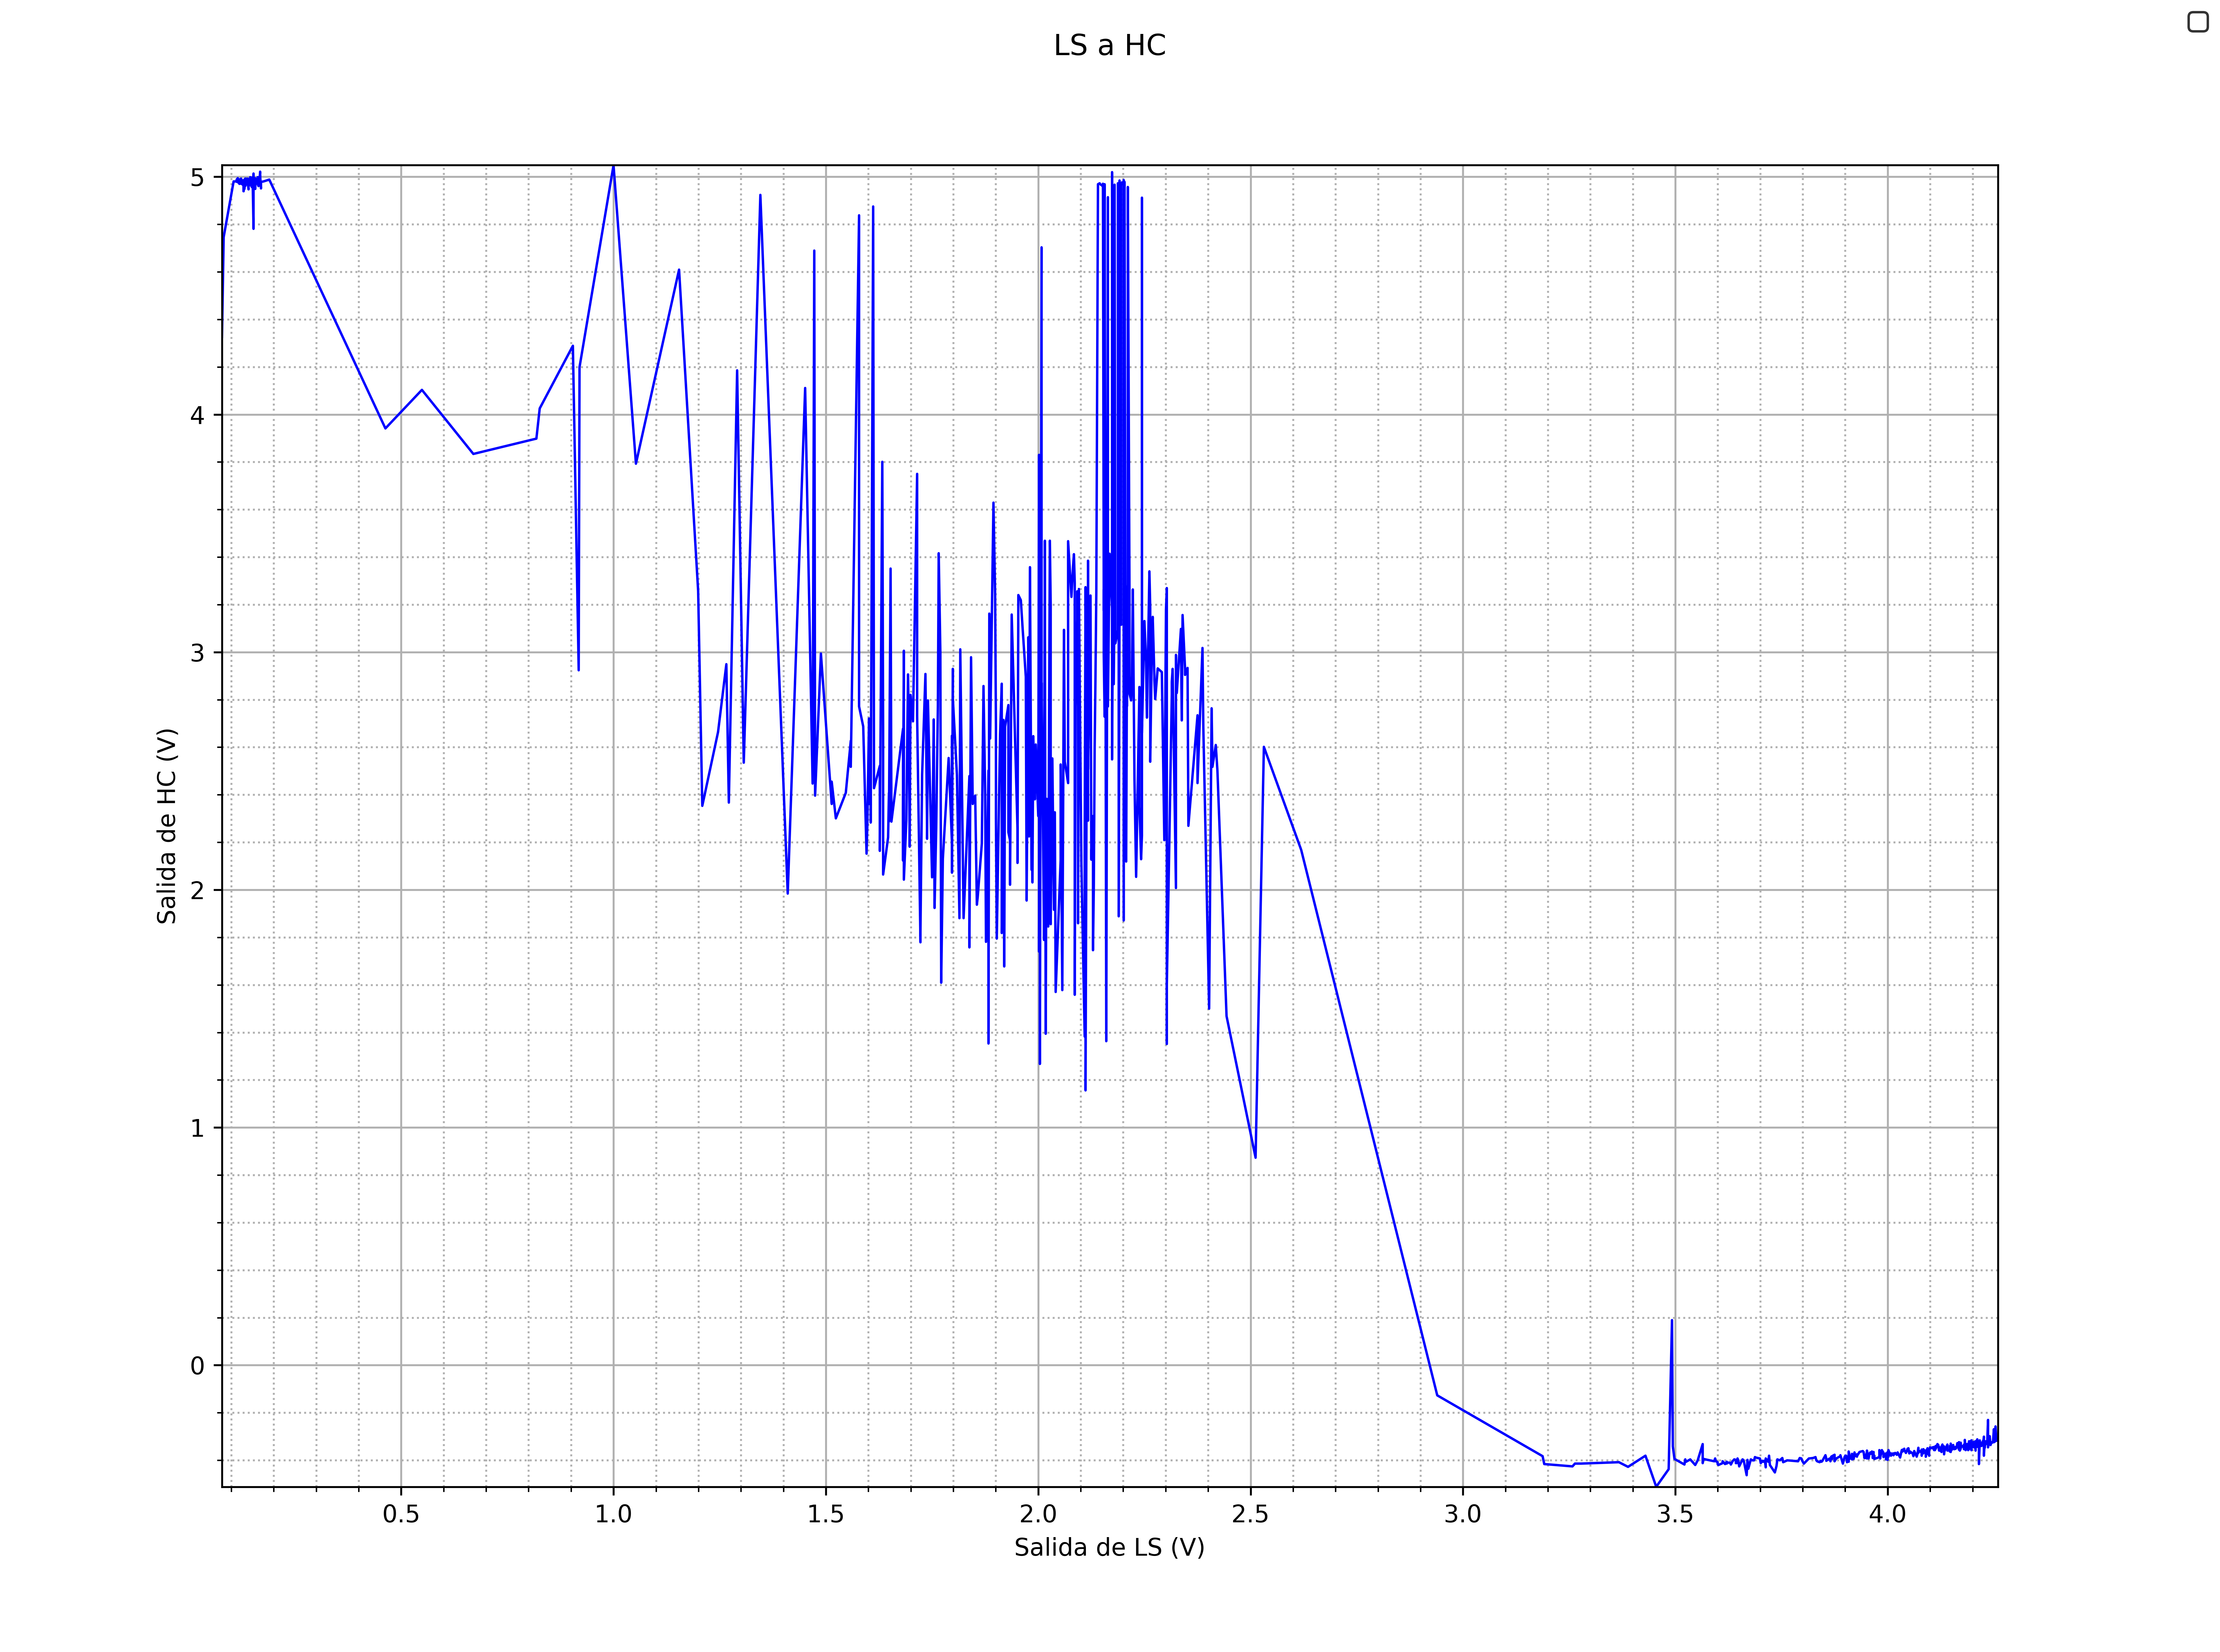
\includegraphics[width=0.5\textwidth]{../EJ2/Recursos/LS_H_v_HC_L}
    \end{tabular}
    \caption{LS a HC, con LS pasando de 1 a 0, y HC de 0 a 1.}
    \label{fig:LS_H_v_HC_L_ex5}
\end{figure}

\begin{figure}[H]
    \centering
    \begin{tabular}{c c}
        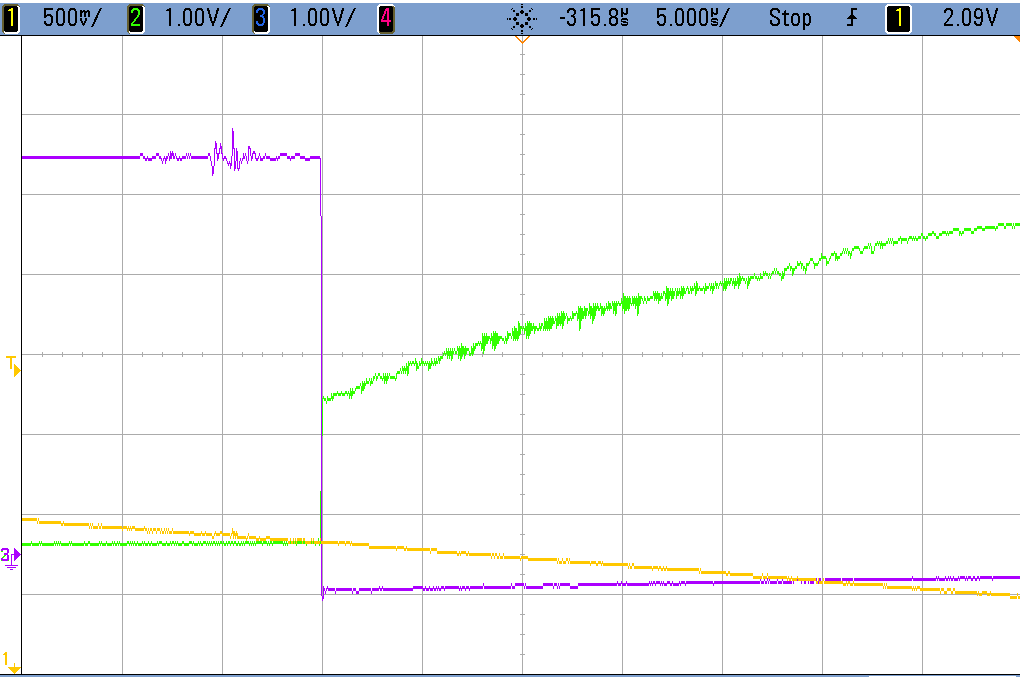
\includegraphics[width=0.5\textwidth]{../EJ2/Recursos/scope_38} &
        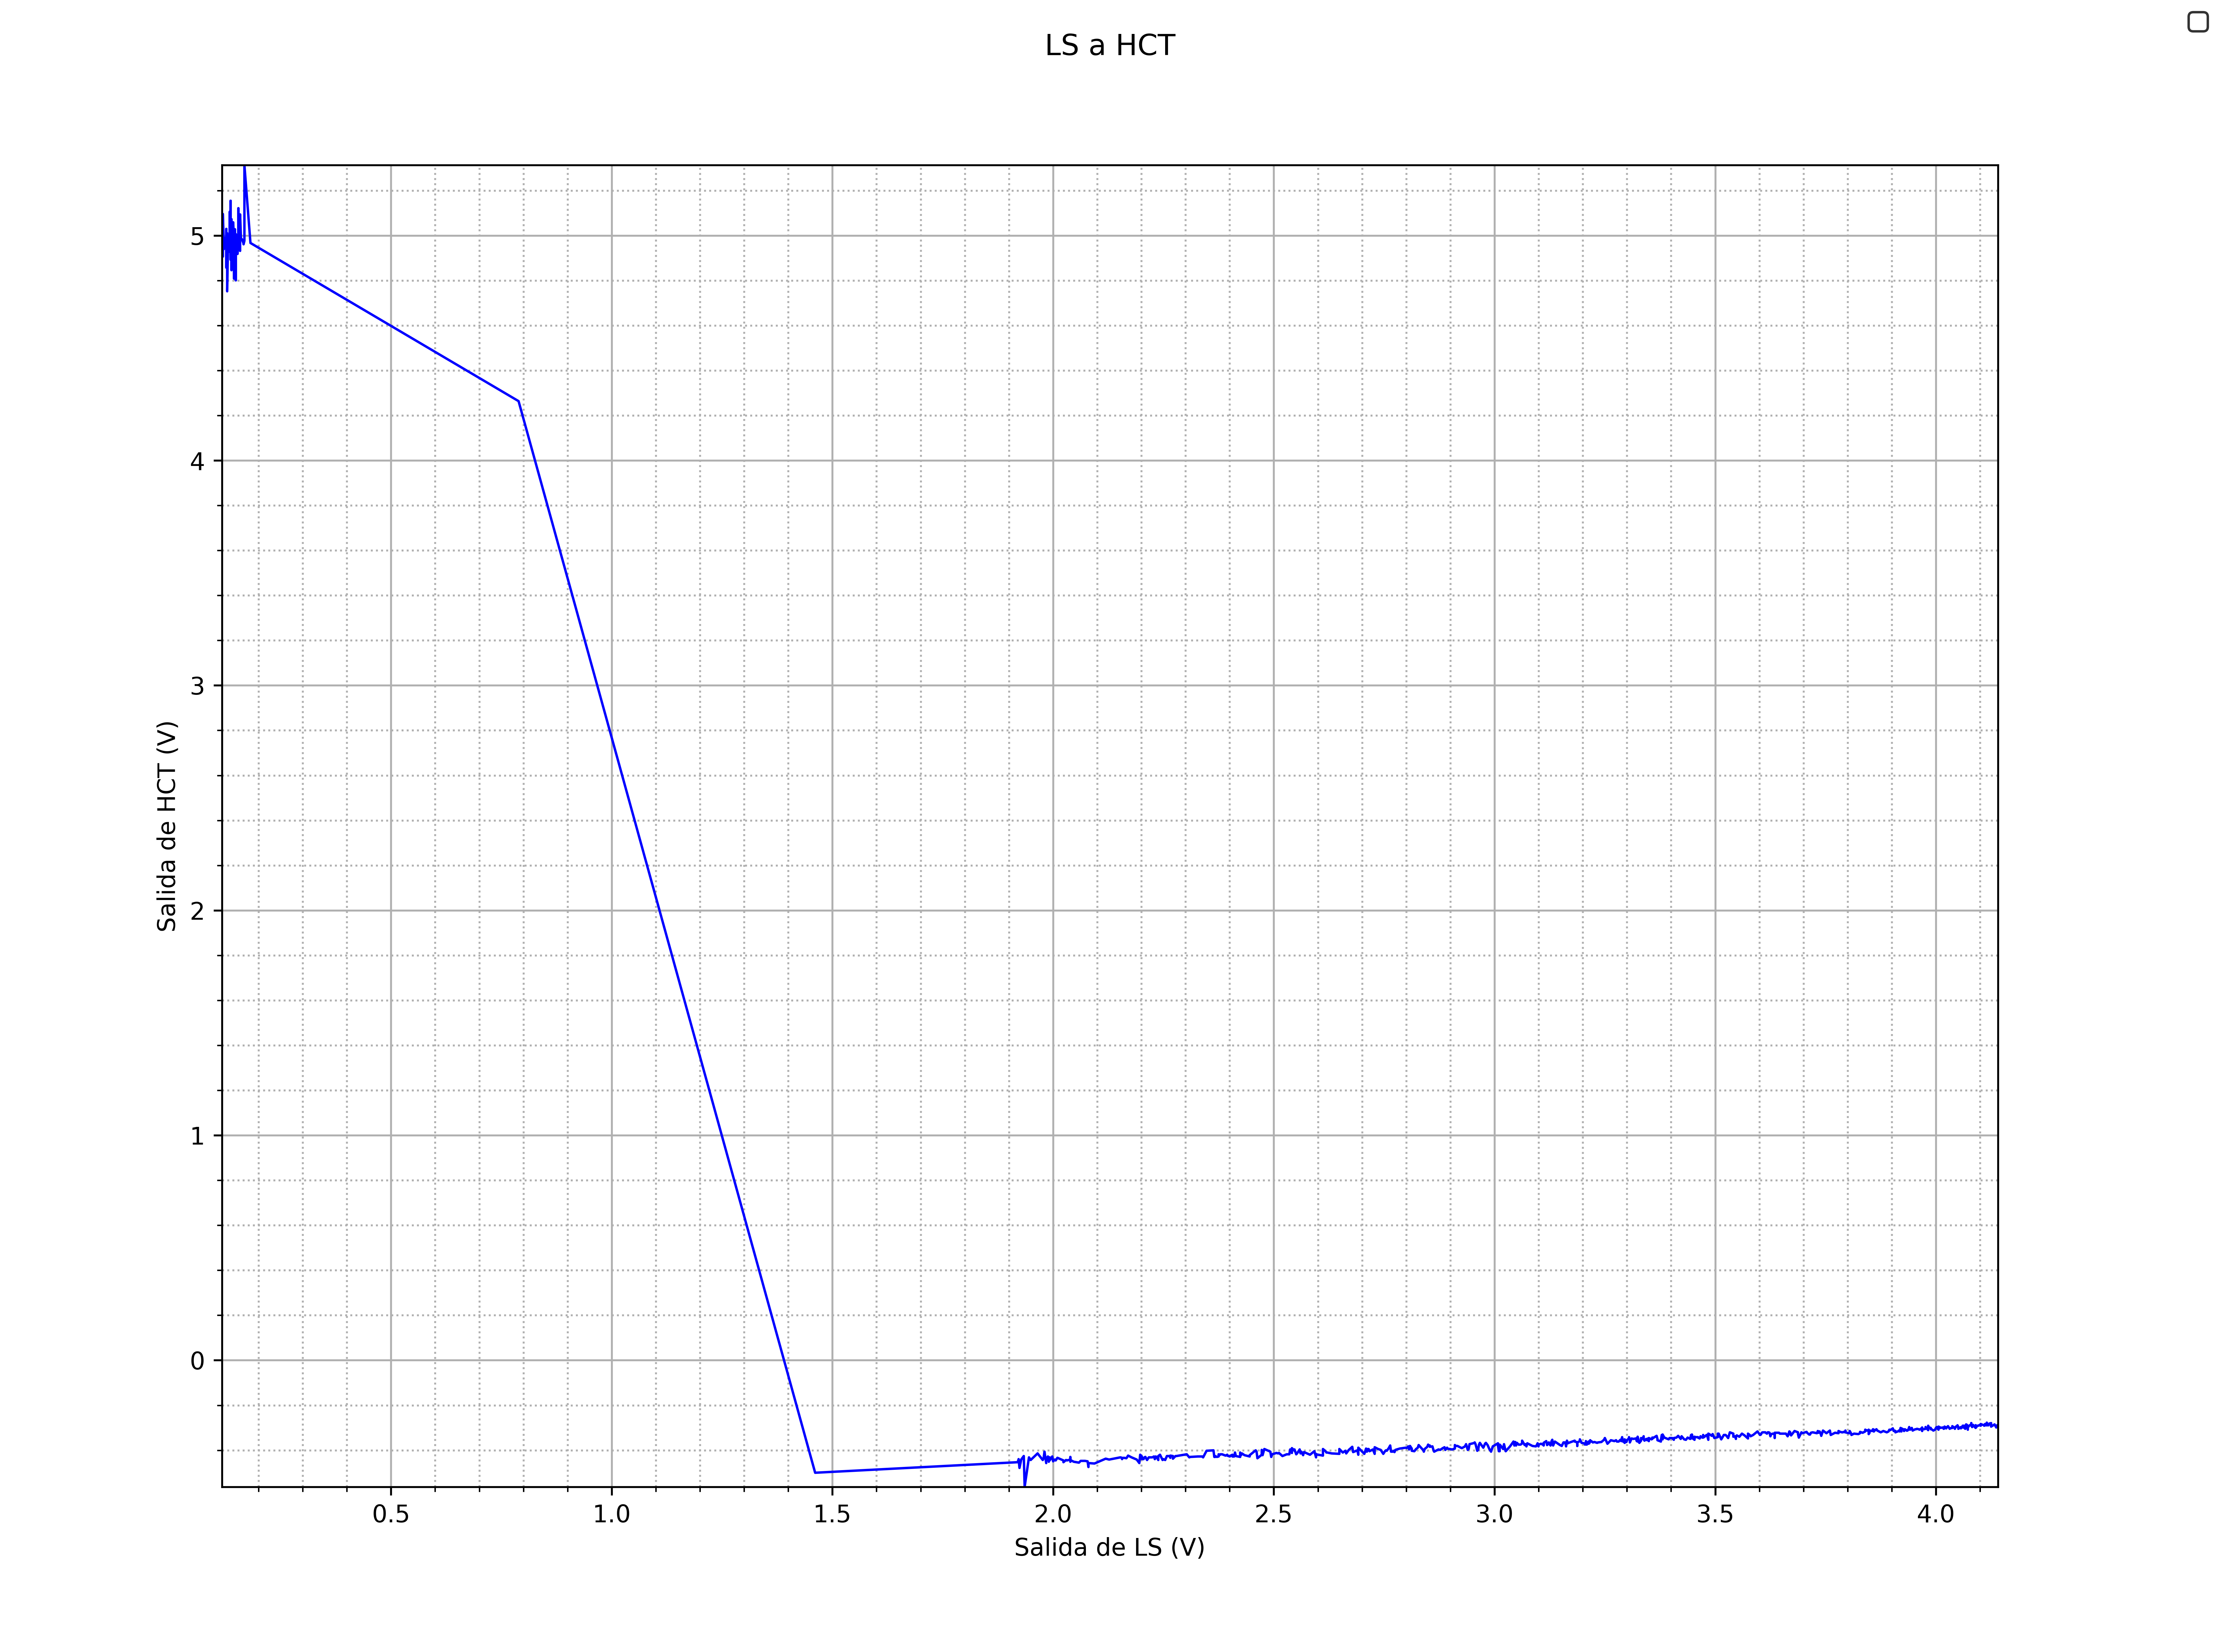
\includegraphics[width=0.5\textwidth]{../EJ2/Recursos/LS_L_v_HCT_H}
    \end{tabular}
    \caption{LS a HCT, con LS pasando de 0 a 1, y HCT de 1 a 0.}
    \label{fig:LS_L_v_HCT_H_ex5}
\end{figure}
\begin{figure}[H]
    \centering
    \begin{tabular}{c c}
        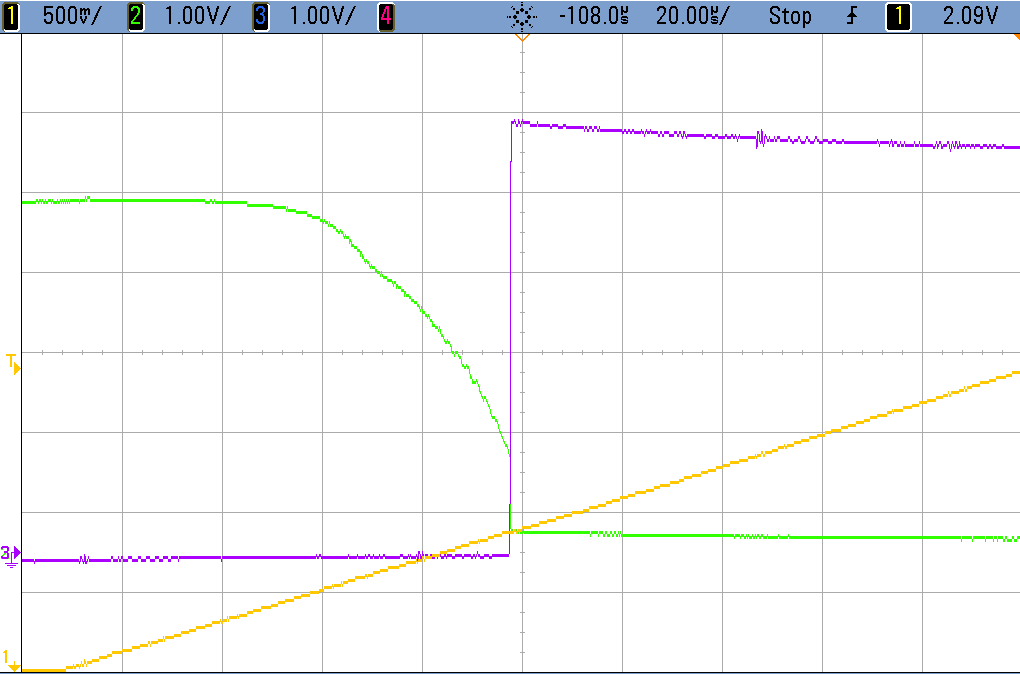
\includegraphics[width=0.5\textwidth]{../EJ2/Recursos/scope_35} &
        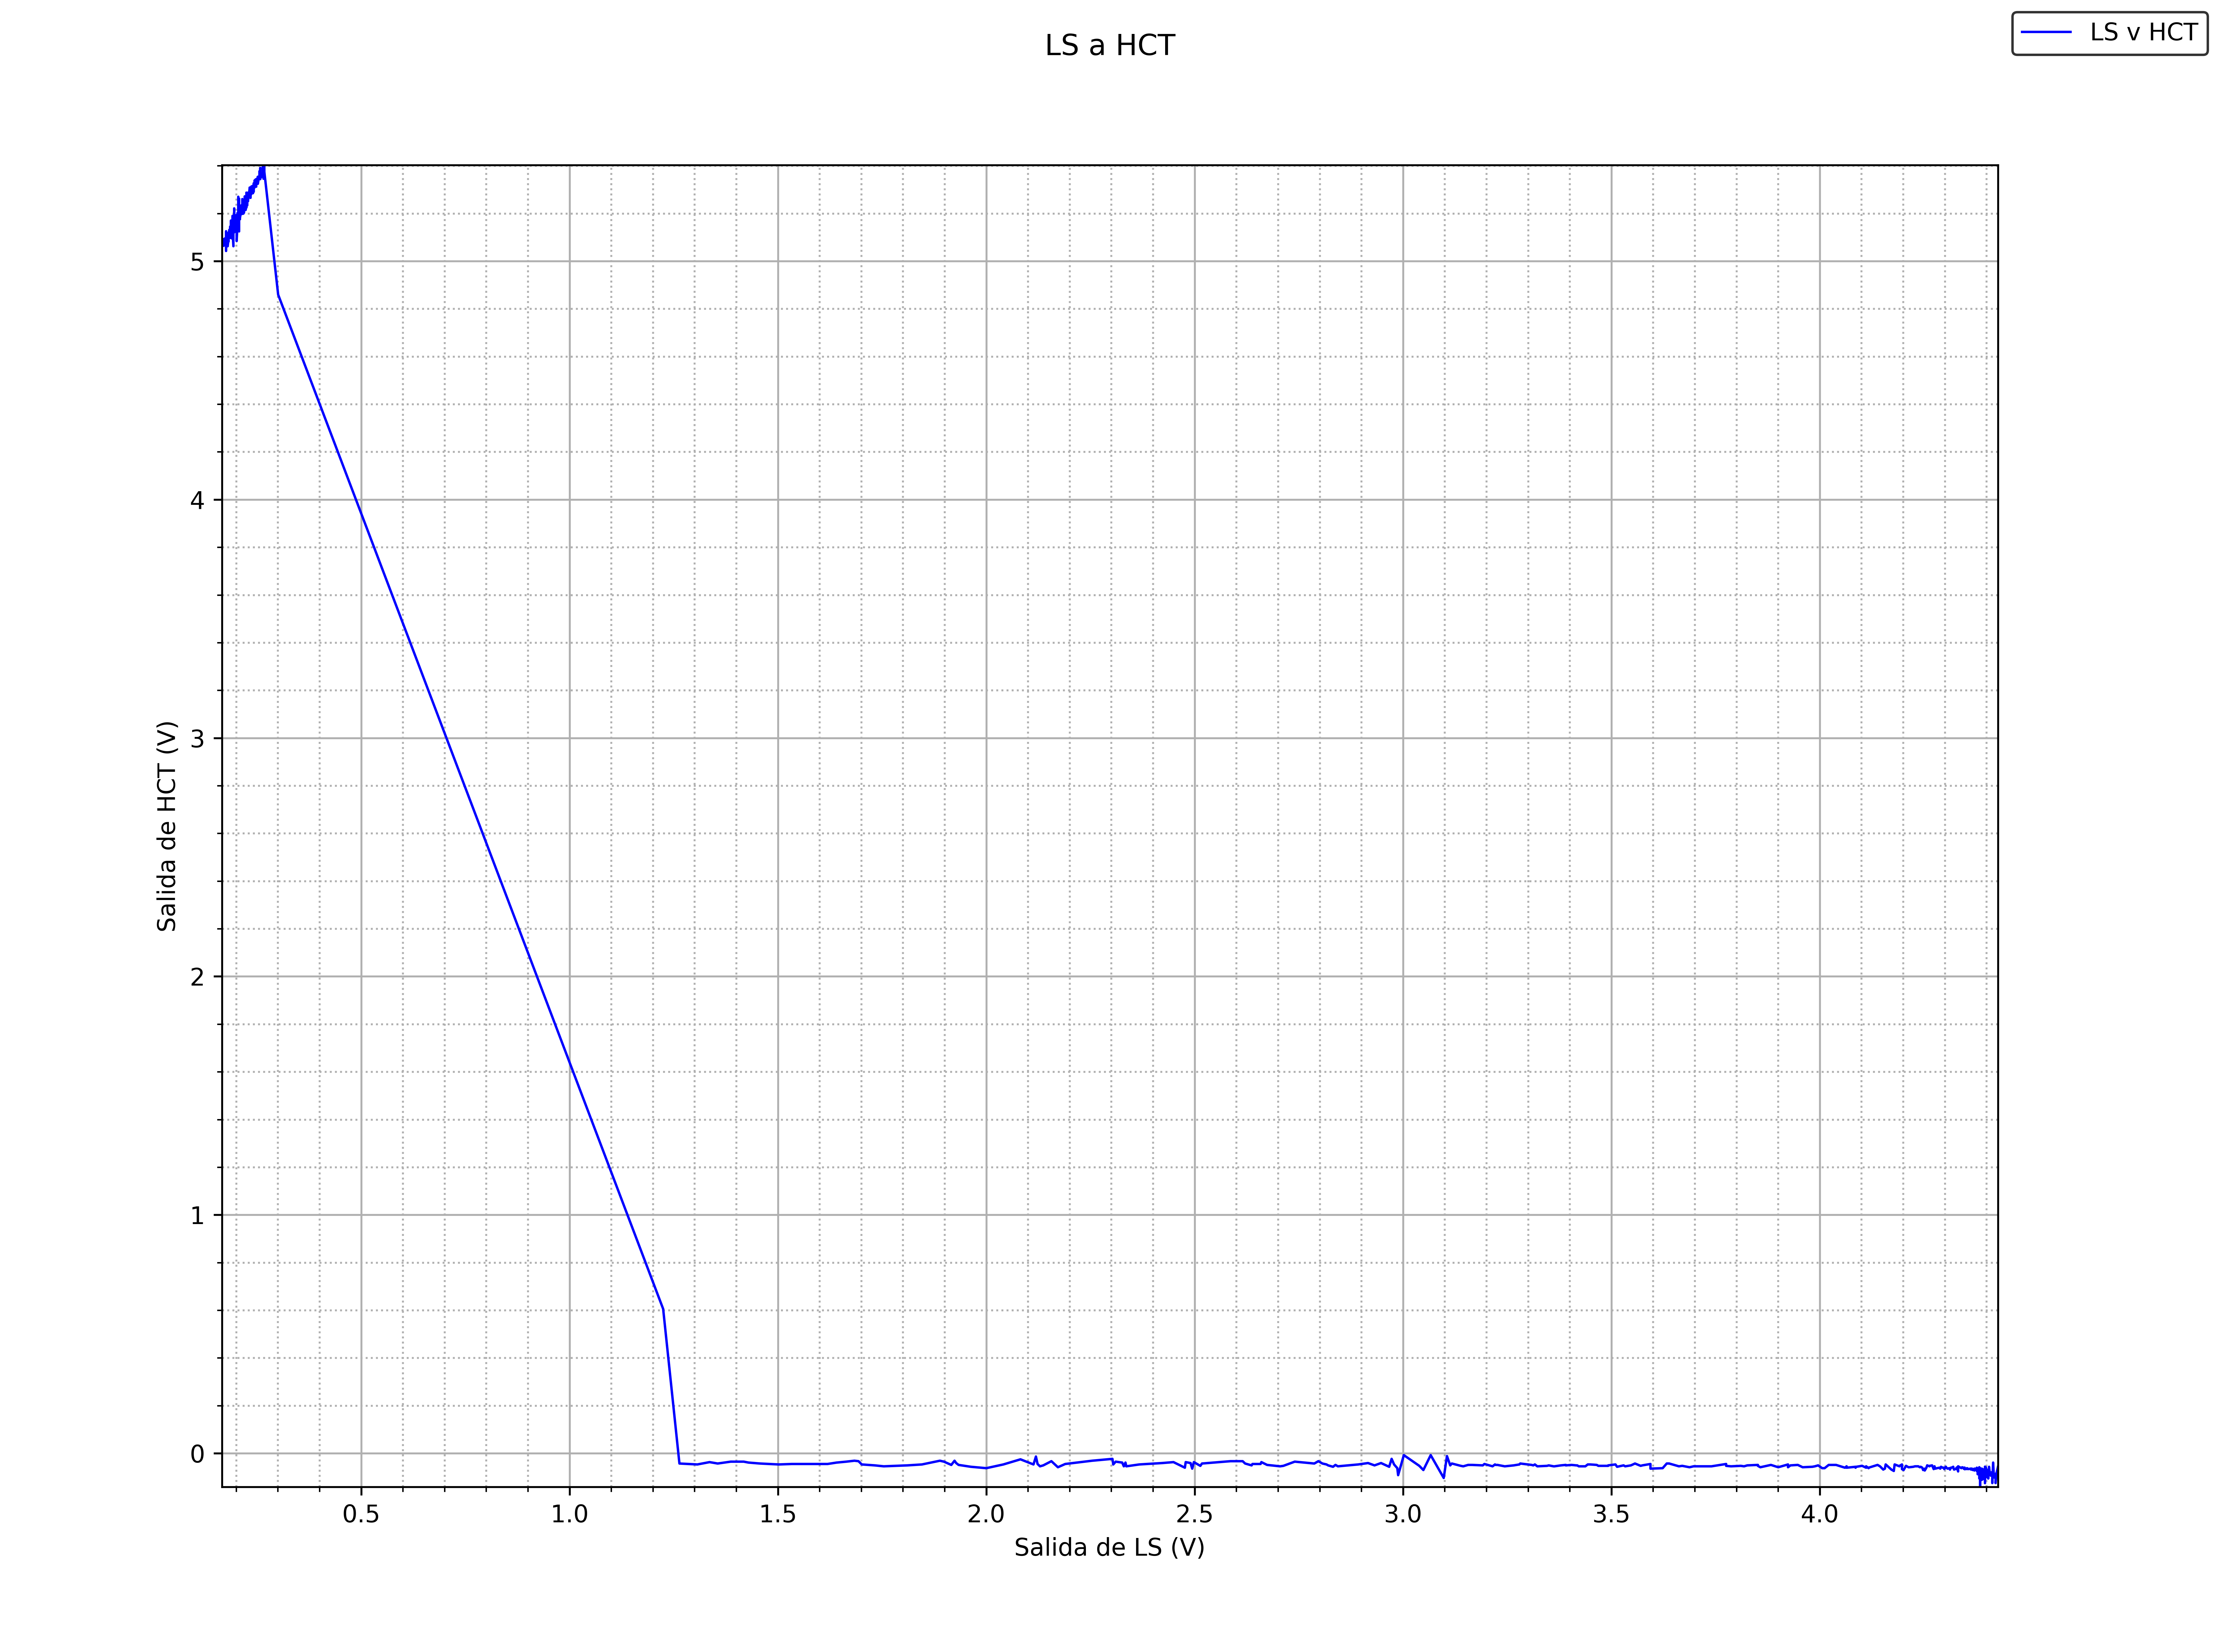
\includegraphics[width=0.5\textwidth]{../EJ2/Recursos/LS_H_v_HCT_L}
    \end{tabular}
    \caption{LS a HCT, con LS pasando de 1 a 0, y HCT de 0 a 1.}
    \label{fig:LS_H_v_HCT_L_ex5}
\end{figure}

Efectivamente lo esperado es lo que se obtiene en las mediciones, donde se puede apreciar una zona de indeterminación y oscilación en las transiciones de la configuración 
LS a HC.
Estos fenómenos no se observan luego en la configuración LS a HCT, en concordancia con lo estudiado de las hojas de datos, donde se aseguraba su compatibilidad.



\subsection{Conclusi\'on}
A modo de cierre, se llega a la conclusión que la compatibilidad de tecnologías es un factor a tener en cuenta a la hora de realizar un diseño con compuertas lógicas de 
más de un tipo, si se quieren evitar estados indeterminados o glitches producto de transiciones con oscilaciones, causadas por incompatibilidades.
Se debe prestar especial atención al paso de tecnologías TTL a CMOS, y de ser necesario implementarlo, debe hacerse uso de compuertas CMOS especialmente diseñadas para 
esa aplicación, como lo son las de tipo HCT.
=======
\section{Ejercicio 2: Comparaci\'on de compuertas discretas con tecnolog\'ia TTL y CMOS}
Se plantea estudiar la compatibilidad de compuertas de tecnología TTL (a base de transistores BJT) con CMOS (transistores MOSFET), enfocando la problemática desde el 
estudio de sus características de márgen de ruido, y haciendo también mención al fanout. 
Se abordará este análisis mediante el estudio de caso de los integrados 74HC02, 74HCT02 y 74LS02, los cuales contienen 4 compuertas NOR cada uno, implementados mediante 
distintas tecnologías.



\subsection{Marco teórico}
Las letras LS en 74LS02 refieren "Low-power Schottky", una tecnología del tipo TTL que alcanza mejores rendimientos y velocidad gracias a la implementación de 
transistores Schottky, los cuales difieren de los clásicos BJT únicamente en el agregado de un diodo Schottky entre sus terminales Base y Colector.
Por otro lado, HC y HCT refieren a "High-speed CMOS", distinguiéndose HCT por ser compatible con las tecnologías TTL.

\begin{figure}[H]
    \centering
    \begin{tabular}{c c}
        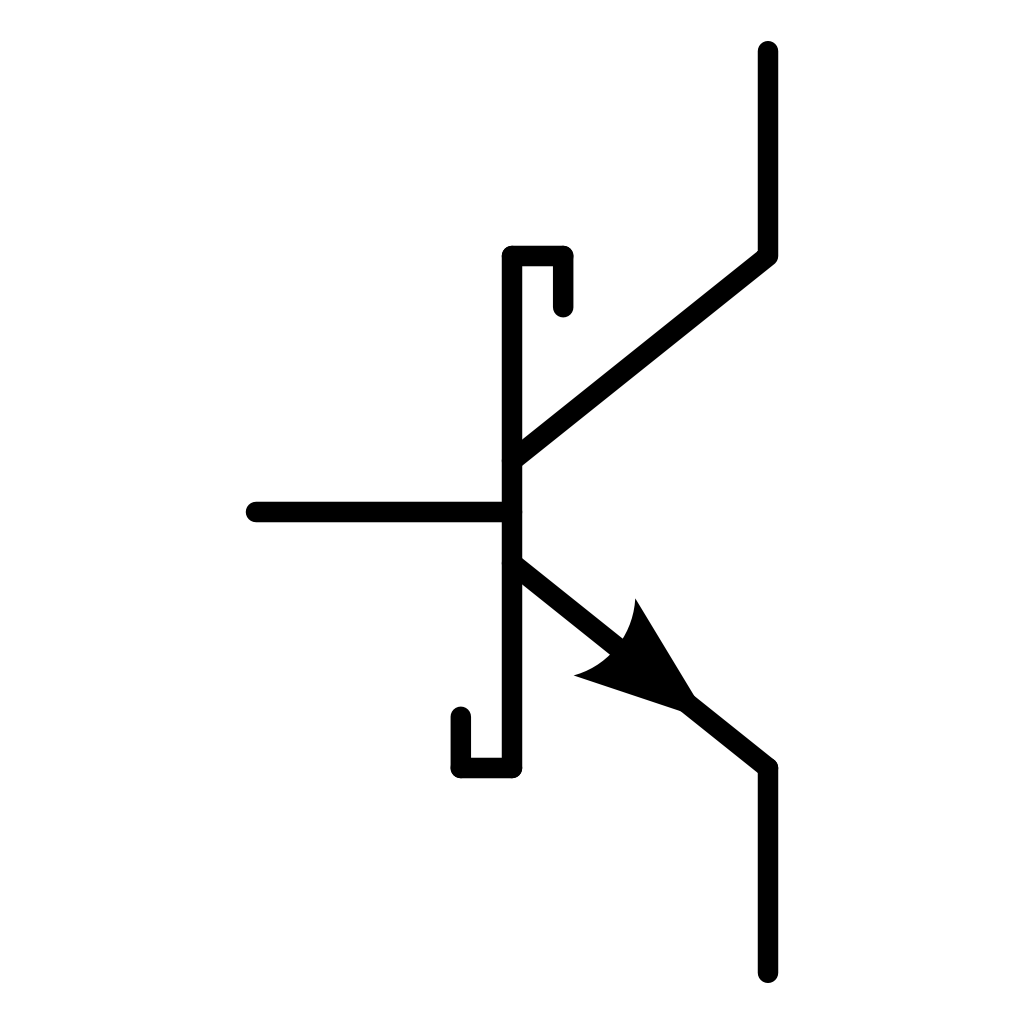
\includegraphics[width=0.1\textwidth]{../EJ2/Recursos/schottky_transistor_symbol} &
        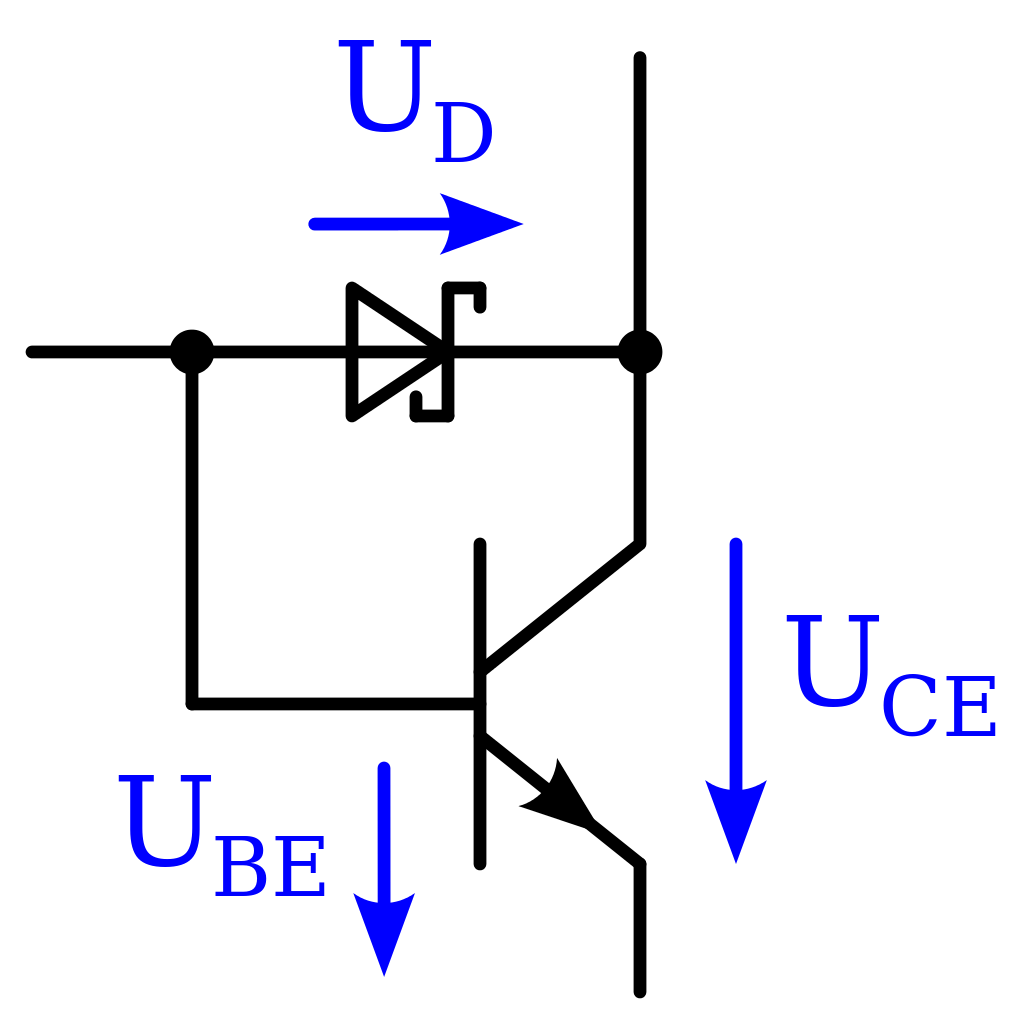
\includegraphics[width=0.1\textwidth]{../EJ2/Recursos/schottky_transistor_circuit}
    \end{tabular}
    \caption{Símbolo y circuito de transistor Schottky.}
    \label{fig:schottky_transistor_symbol_and_circuit_ex5}
\end{figure}

Tal y como fue mencionado en el inicio de esta sección, en este trabajo se estudiará la compatibilidad entre las tecnologías a través de sus márgenes de ruido.
Esto significa que, en términos de interconexión, una compuerta solo será compatible con otra de otra tecnología, si el rango de valores de salida de la primera está 
incluido en el rango de entrada de la segunda. \\
En las figuras \ref{fig:compatible_v_non_compatible_ex5} y \ref{fig:compatible_v_non_compatible_2_ex5} pueden apreciarse los casos que pueden presentarse que significarán la compatibilidad o no entre las compuertas.
De ellos se extrae que las compuertas serán compatibles solo en el caso en que $V_{OH} \geq V_{IH}$ y $V_{OL} \leq V_{IL}$.

\begin{figure}[H]
    \centering
    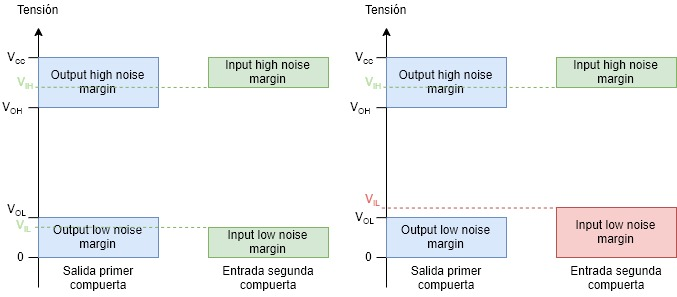
\includegraphics[width=0.9\textwidth]{../EJ2/Recursos/compatible_gates}
    \caption{Compatibilidad de compuertas.}
    \label{fig:compatible_v_non_compatible_ex5}
\end{figure}

\begin{figure}[H]
    \centering
    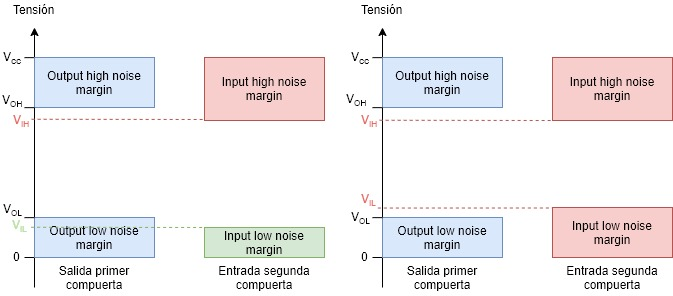
\includegraphics[width=0.9\textwidth]{../EJ2/Recursos/incompatible_gates}
    \caption{Compatibilidad de compuertas.}
    \label{fig:compatible_v_non_compatible_2_ex5}
\end{figure}

Con respecto al fanout, el mismo es una limitación para la cantidad de compuertas que se pueden colocar a la salida de otra, que viene dada por las corrientes de entrada 
y salida, respectivamente.

\begin{equation}
    fanout = min\left(\frac{I_{OH}}{I_{IH}} ; \frac{I_{OL}}{I_{IL}}\right)
\end{equation}



\subsection{Análisis mediante hojas de datos}
Se estudia la compatibilidad de la interconexión de las compuertas mediante la observación de las hojas de datos de los integrados 
74HC02\footnote{http://pdf.datasheetcatalog.com/datasheet/NXP\_Semiconductors/74HC\_HCT02.pdf}, 74HCT02\footnote{http://pdf.datasheetcatalog.com/datasheet/NXP\_Semiconductors/74HC\_HCT02.pdf} y 74LS02\footnote{http://www.sycelectronica.com.ar/semiconductores/74LS02.pdf},
y se exponen los datos utilizados en la tabla \ref{table:parameters_datasheet_ex5}.
Cabe mencionar que las condiciones de prueba de estos parámetros no son las mismas para las compuertas de tecnología CMOS que para las de TTL, de modo que se decide tomar 
el caso más desfavorable para cada una de las comparaciones.
En todos los casos, este terminó siendo que para las compuertas HC y HCT, la alimentación es de $4,5 V$, mientras que para las LS es de $5 V$.

\begin{table}[H]
    \begin{tabular}{ccccccccc}
    \textbf{Integrado} & \textbf{$V_{OH}$} & \textbf{$V_{OL}$} & \textbf{$V_{IH}$} & \textbf{$V_{IL}$} & \textbf{$I_{OH}$} & \textbf{$I_{OL}$} & \textbf{$I_{IH}$} & \textbf{$I_{IL}$} \\ \hline
    \textbf{74HC02}    & $4,4 V$           & $0,1 V$           & $3,15 V$          & $1,35 V$          & $\pm 25 mA$       & $\pm 25 mA$       & $\pm 0,1 \mu A$   & $\pm 0,1 \mu A$   \\
    \textbf{74HCT02}   & $4,4 V$           & $0,1 V$           & $2 V$             & $0,8 V$           & $\pm 25 mA$       & $\pm 25 mA$       & $\pm 0,1 \mu A$   & $\pm 0,1 \mu A$   \\
    \textbf{74LS02}    & $2,7 V$           & $0,5 V$           & $2 V$             & $0,8 V$           & $-0,4 mA$         & $8 mA$            & $20 \mu A$        & $-0,4 mA$        
    \end{tabular}
    \caption{Parámetros de compatibilidad obtenidos de datasheet.}
    \label{table:parameters_datasheet_ex5}
\end{table}

Se desprende de los datos expuestos y de la teoría explicada en el marco teórico, que son compatibles las conexiones de una compuerta HC a LS, de una HCT a LS, y de una 
LS a una HCT, ya que en todos estos casos se cumple que $V_{OH} \geq V_{IH}$ y $V_{OL} \leq V_{IL}$.
También es este el caso entre HCT y HC, y viceversa, resultado que es de esperar ya que comparten el tipo de tecnología.
Sin embargo, no sucede esto al ir de una LS a una HC ya que para esta combinación $V_{OH} < V_{IH}$, quedando una zona de indeterminación entre los valores de tensión 
$2,7 V$ y $3,15 V$.
Esta incompatibilidad es lógicamente salvada al usar tecnología HCT, la cual está diseñada con el propósito de lograr la compatibilidad que carecen las compuertas HC 
entre tecnologías TTL y CMOS.\\
En lo que respecta al fanout, los resultados son los expuestos en la tabla \ref{table:fanout_results_ex5}
\begin{table}[H]
    \begin{tabular}{ccccccc}
    \textbf{Interconexión} & \textbf{HC a LS} & \textbf{LS a HC} & \textbf{HCT a LS} & \textbf{LS a HCT} & \textbf{HC a HCT} & \textbf{HCT a HC} \\ \hline
    \textbf{fanout}        & $62$             & $4000$           & $62$              & $4000$            & $250 \cdot 10^3$  & $250 \cdot 10^3$ 
    \end{tabular}
    \caption{Fanout para distintas conexiones.}
    \label{table:fanout_results_ex5}
\end{table}



\subsection{Resultados experimentales}
Para el caso donde las hojas de datos no aseguran el correcto funcionamiento de la interconexión de compuertas, es decir, de una LS a una HC, se procede a estudiar su 
respuesta de forma experimental.
Se alimenta una compuerta del 74LS02 utilizada como NOT (cortocircuitando sus dos entradas) con una función rampa de 0 a 5V, y a su salida se conecta una del 74HC02, 
también como NOT. 
Se miden las salidas de ambas y los resultados son los expuestos en las figuras \ref{fig:LS_L_v_HC_H_ex5} y \ref{fig:LS_H_v_HC_L_ex5}.\\
Luego se realiza el mismo procedimiento pero en el lugar del 74HC02 se coloca el 74HCT02, cuyos resultados son los de las figuras \ref{fig:LS_L_v_HCT_H_ex5} y \ref{fig:LS_H_v_HCT_L_ex5}.
Se esperan observar indeterminaciones para la primer interconexión, y que tales problemas se vean resueltos al cambiar la tecnología HC por HCT. 

\begin{figure}[H]
    \centering
    \begin{tabular}{c c}
        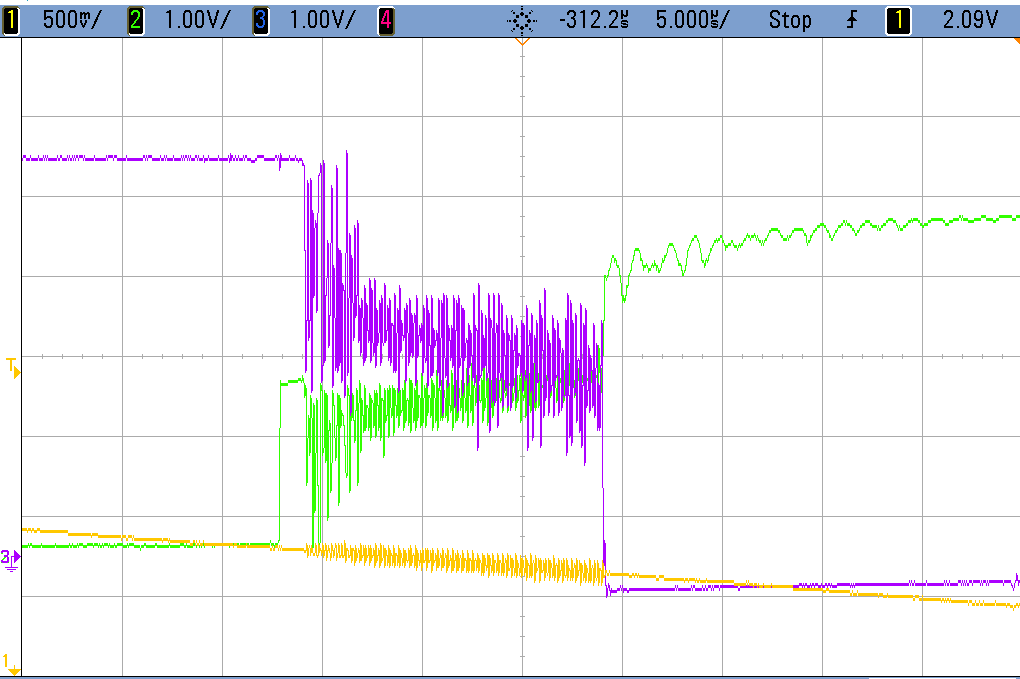
\includegraphics[width=0.5\textwidth]{../EJ2/Recursos/scope_32} &
        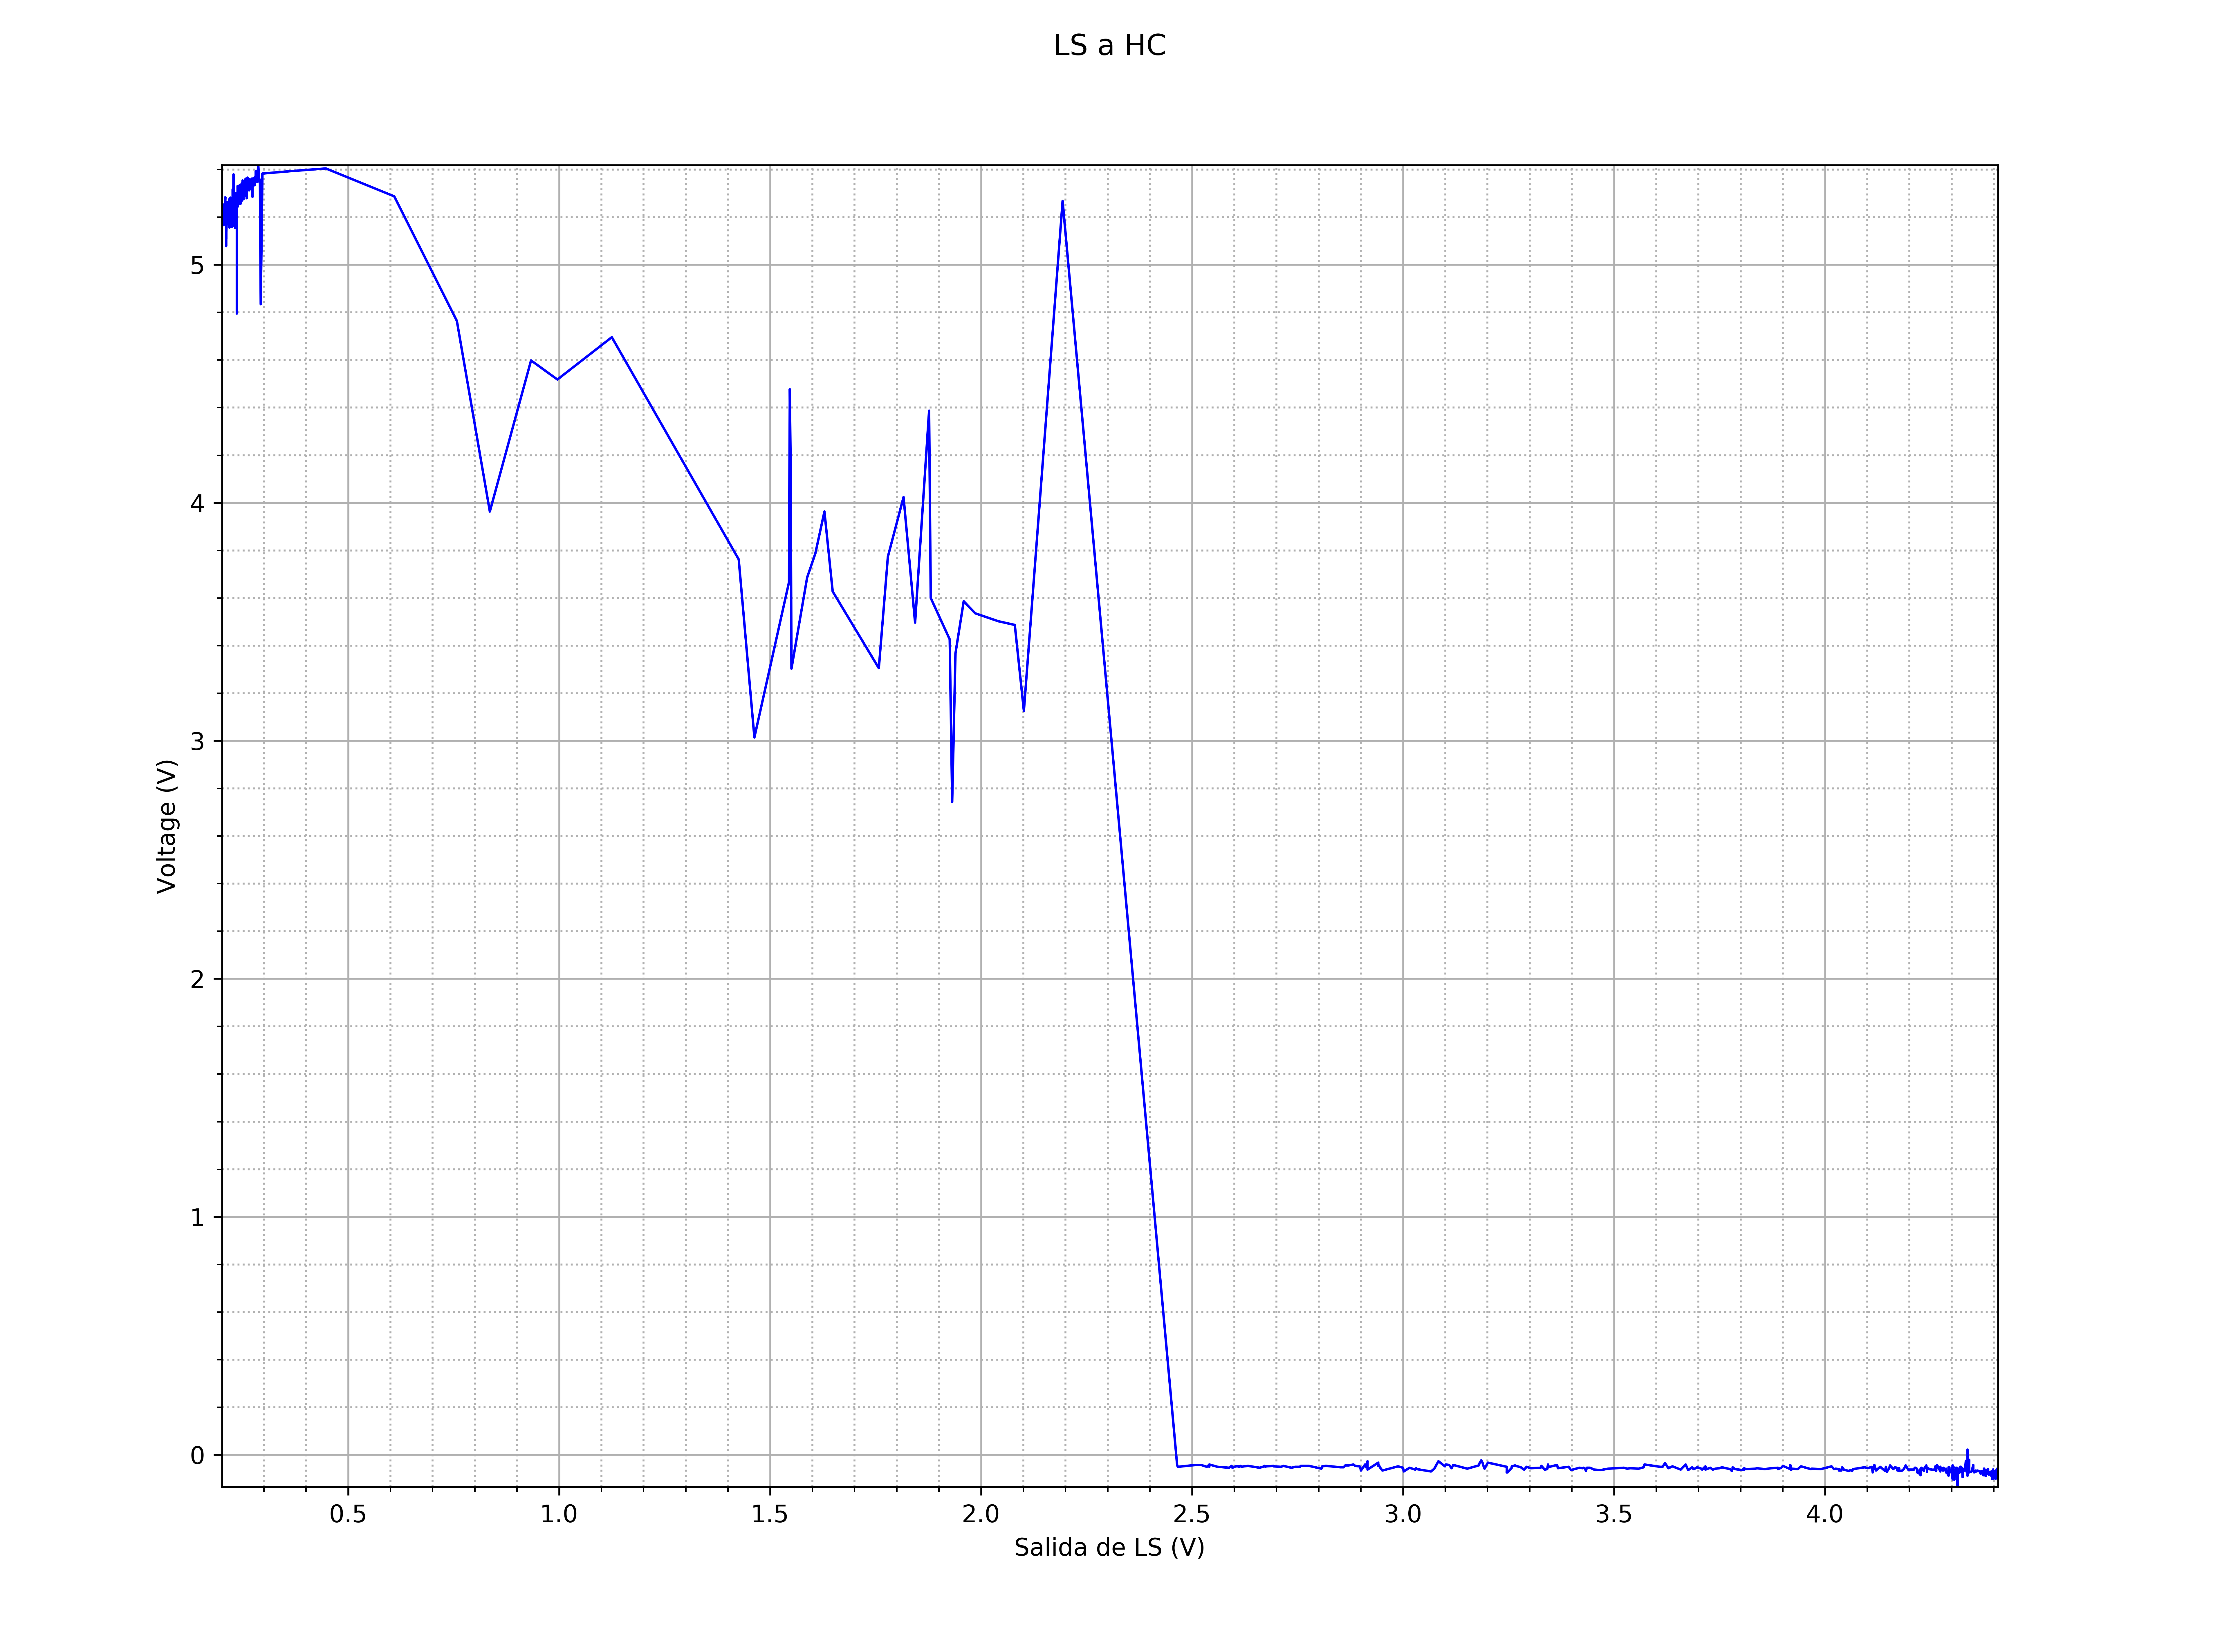
\includegraphics[width=0.5\textwidth]{../EJ2/Recursos/LS_L_v_HC_H}
    \end{tabular}
    \caption{LS a HC, con LS pasando de 0 a 1, y HC de 1 a 0.}
    \label{fig:LS_L_v_HC_H_ex5}
\end{figure}
\begin{figure}[H]
    \centering
    \begin{tabular}{c c}
        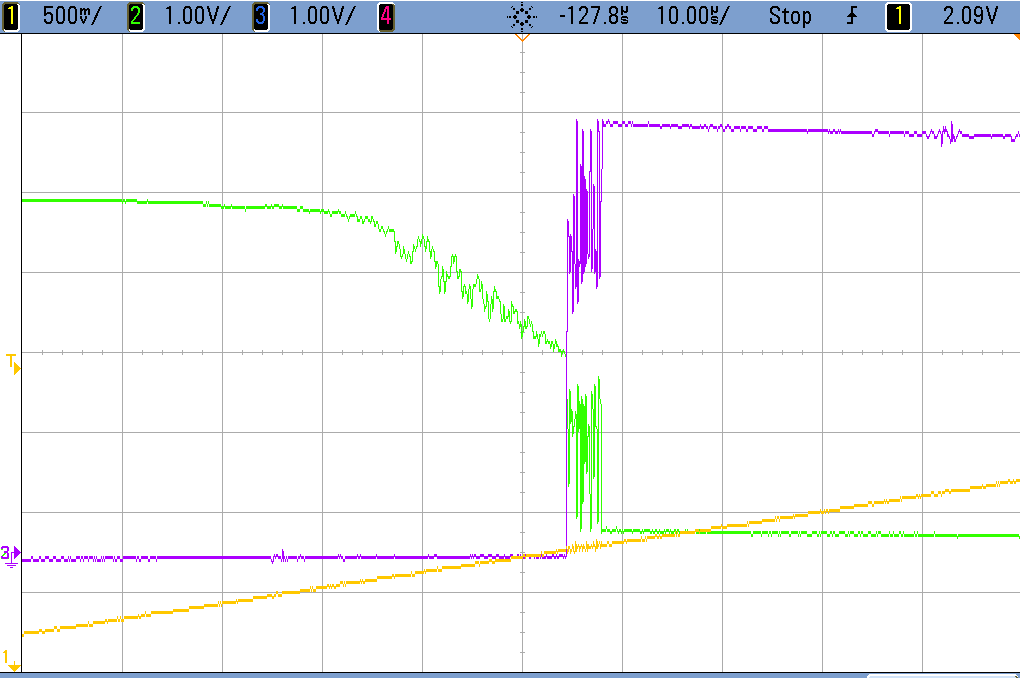
\includegraphics[width=0.5\textwidth]{../EJ2/Recursos/scope_29} &
        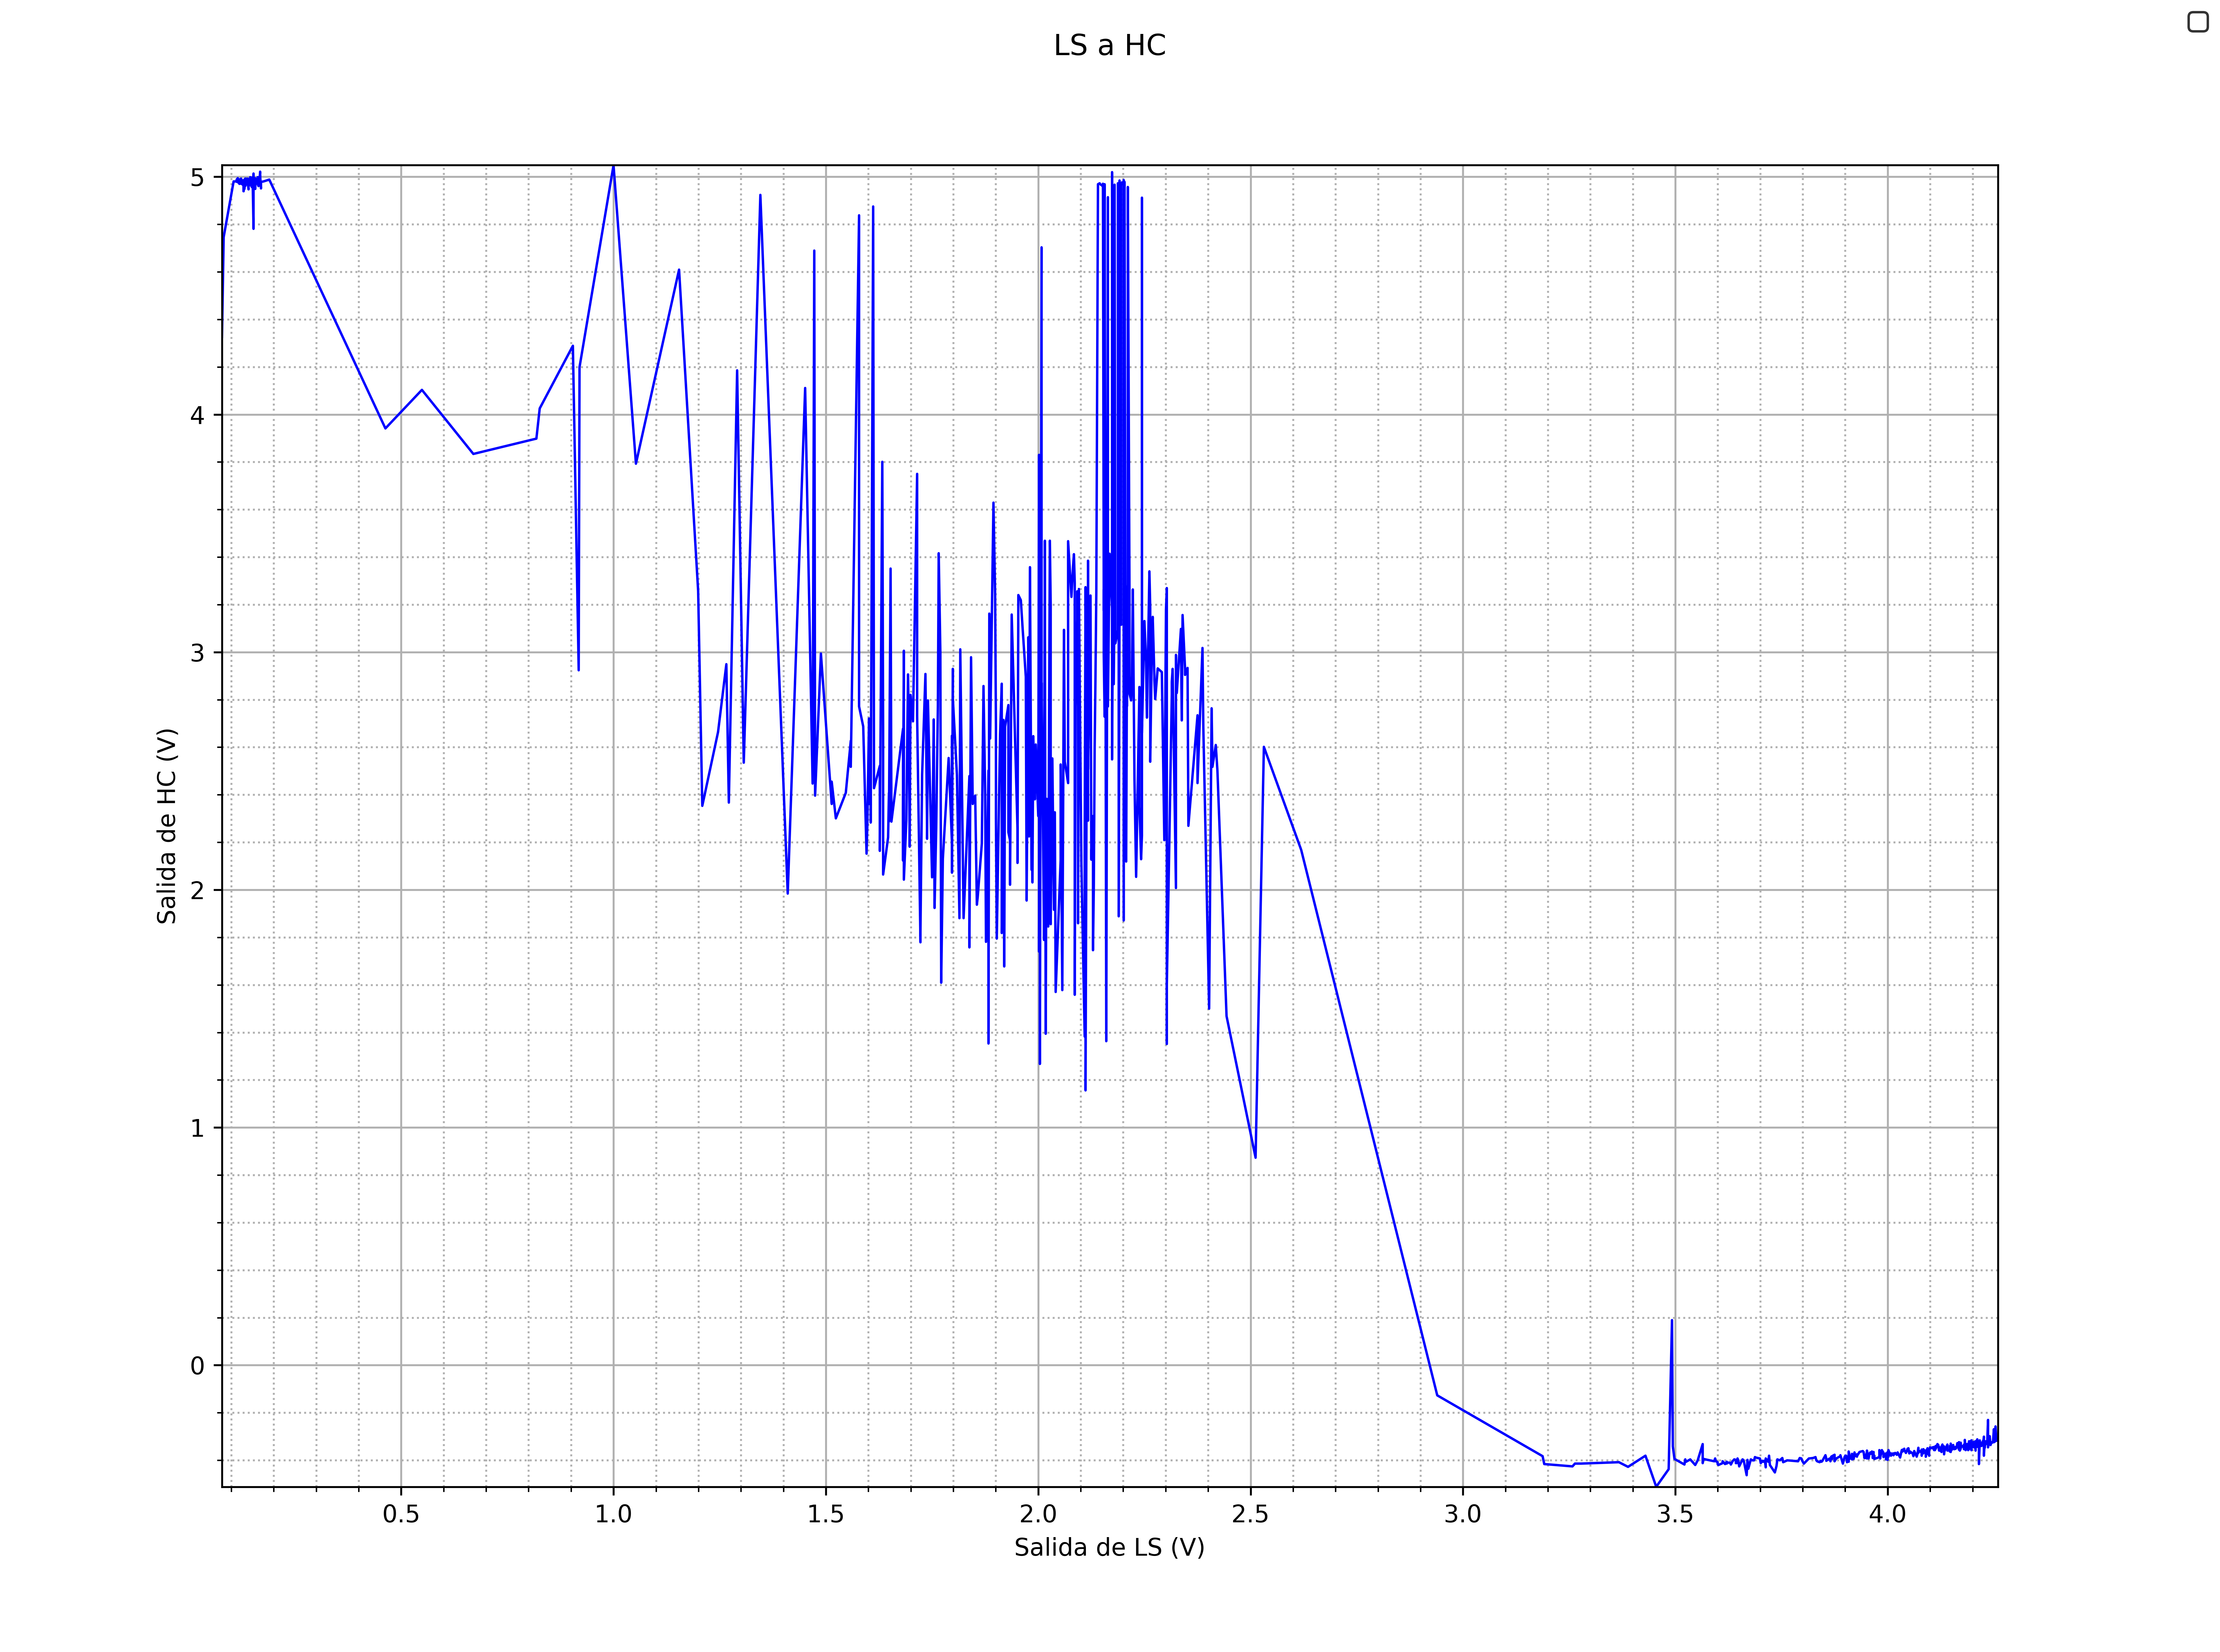
\includegraphics[width=0.5\textwidth]{../EJ2/Recursos/LS_H_v_HC_L}
    \end{tabular}
    \caption{LS a HC, con LS pasando de 1 a 0, y HC de 0 a 1.}
    \label{fig:LS_H_v_HC_L_ex5}
\end{figure}

\begin{figure}[H]
    \centering
    \begin{tabular}{c c}
        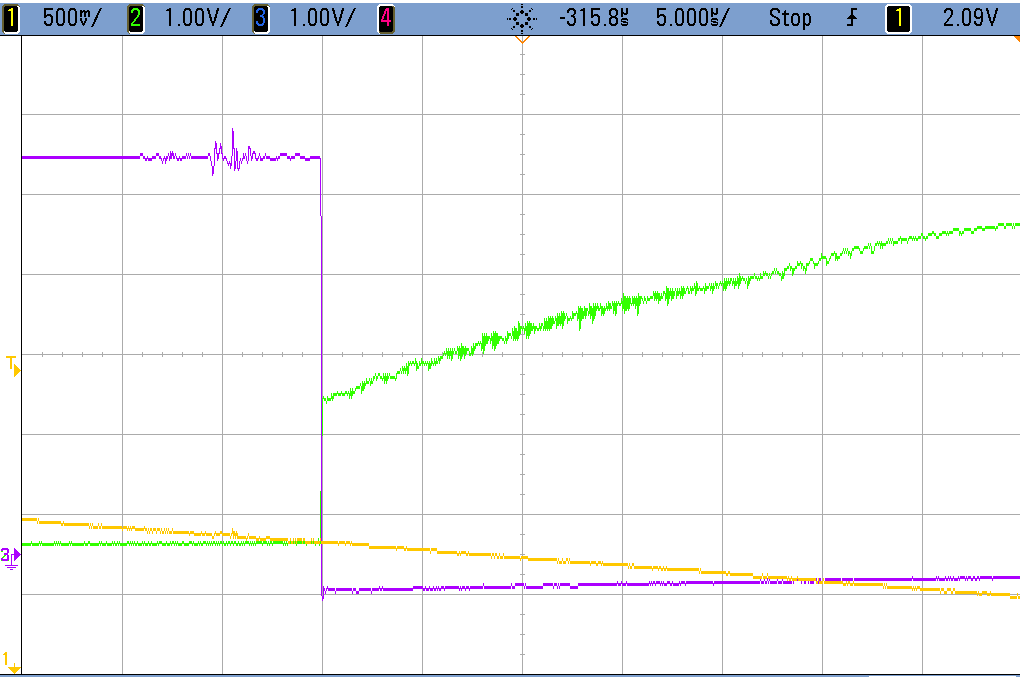
\includegraphics[width=0.5\textwidth]{../EJ2/Recursos/scope_38} &
        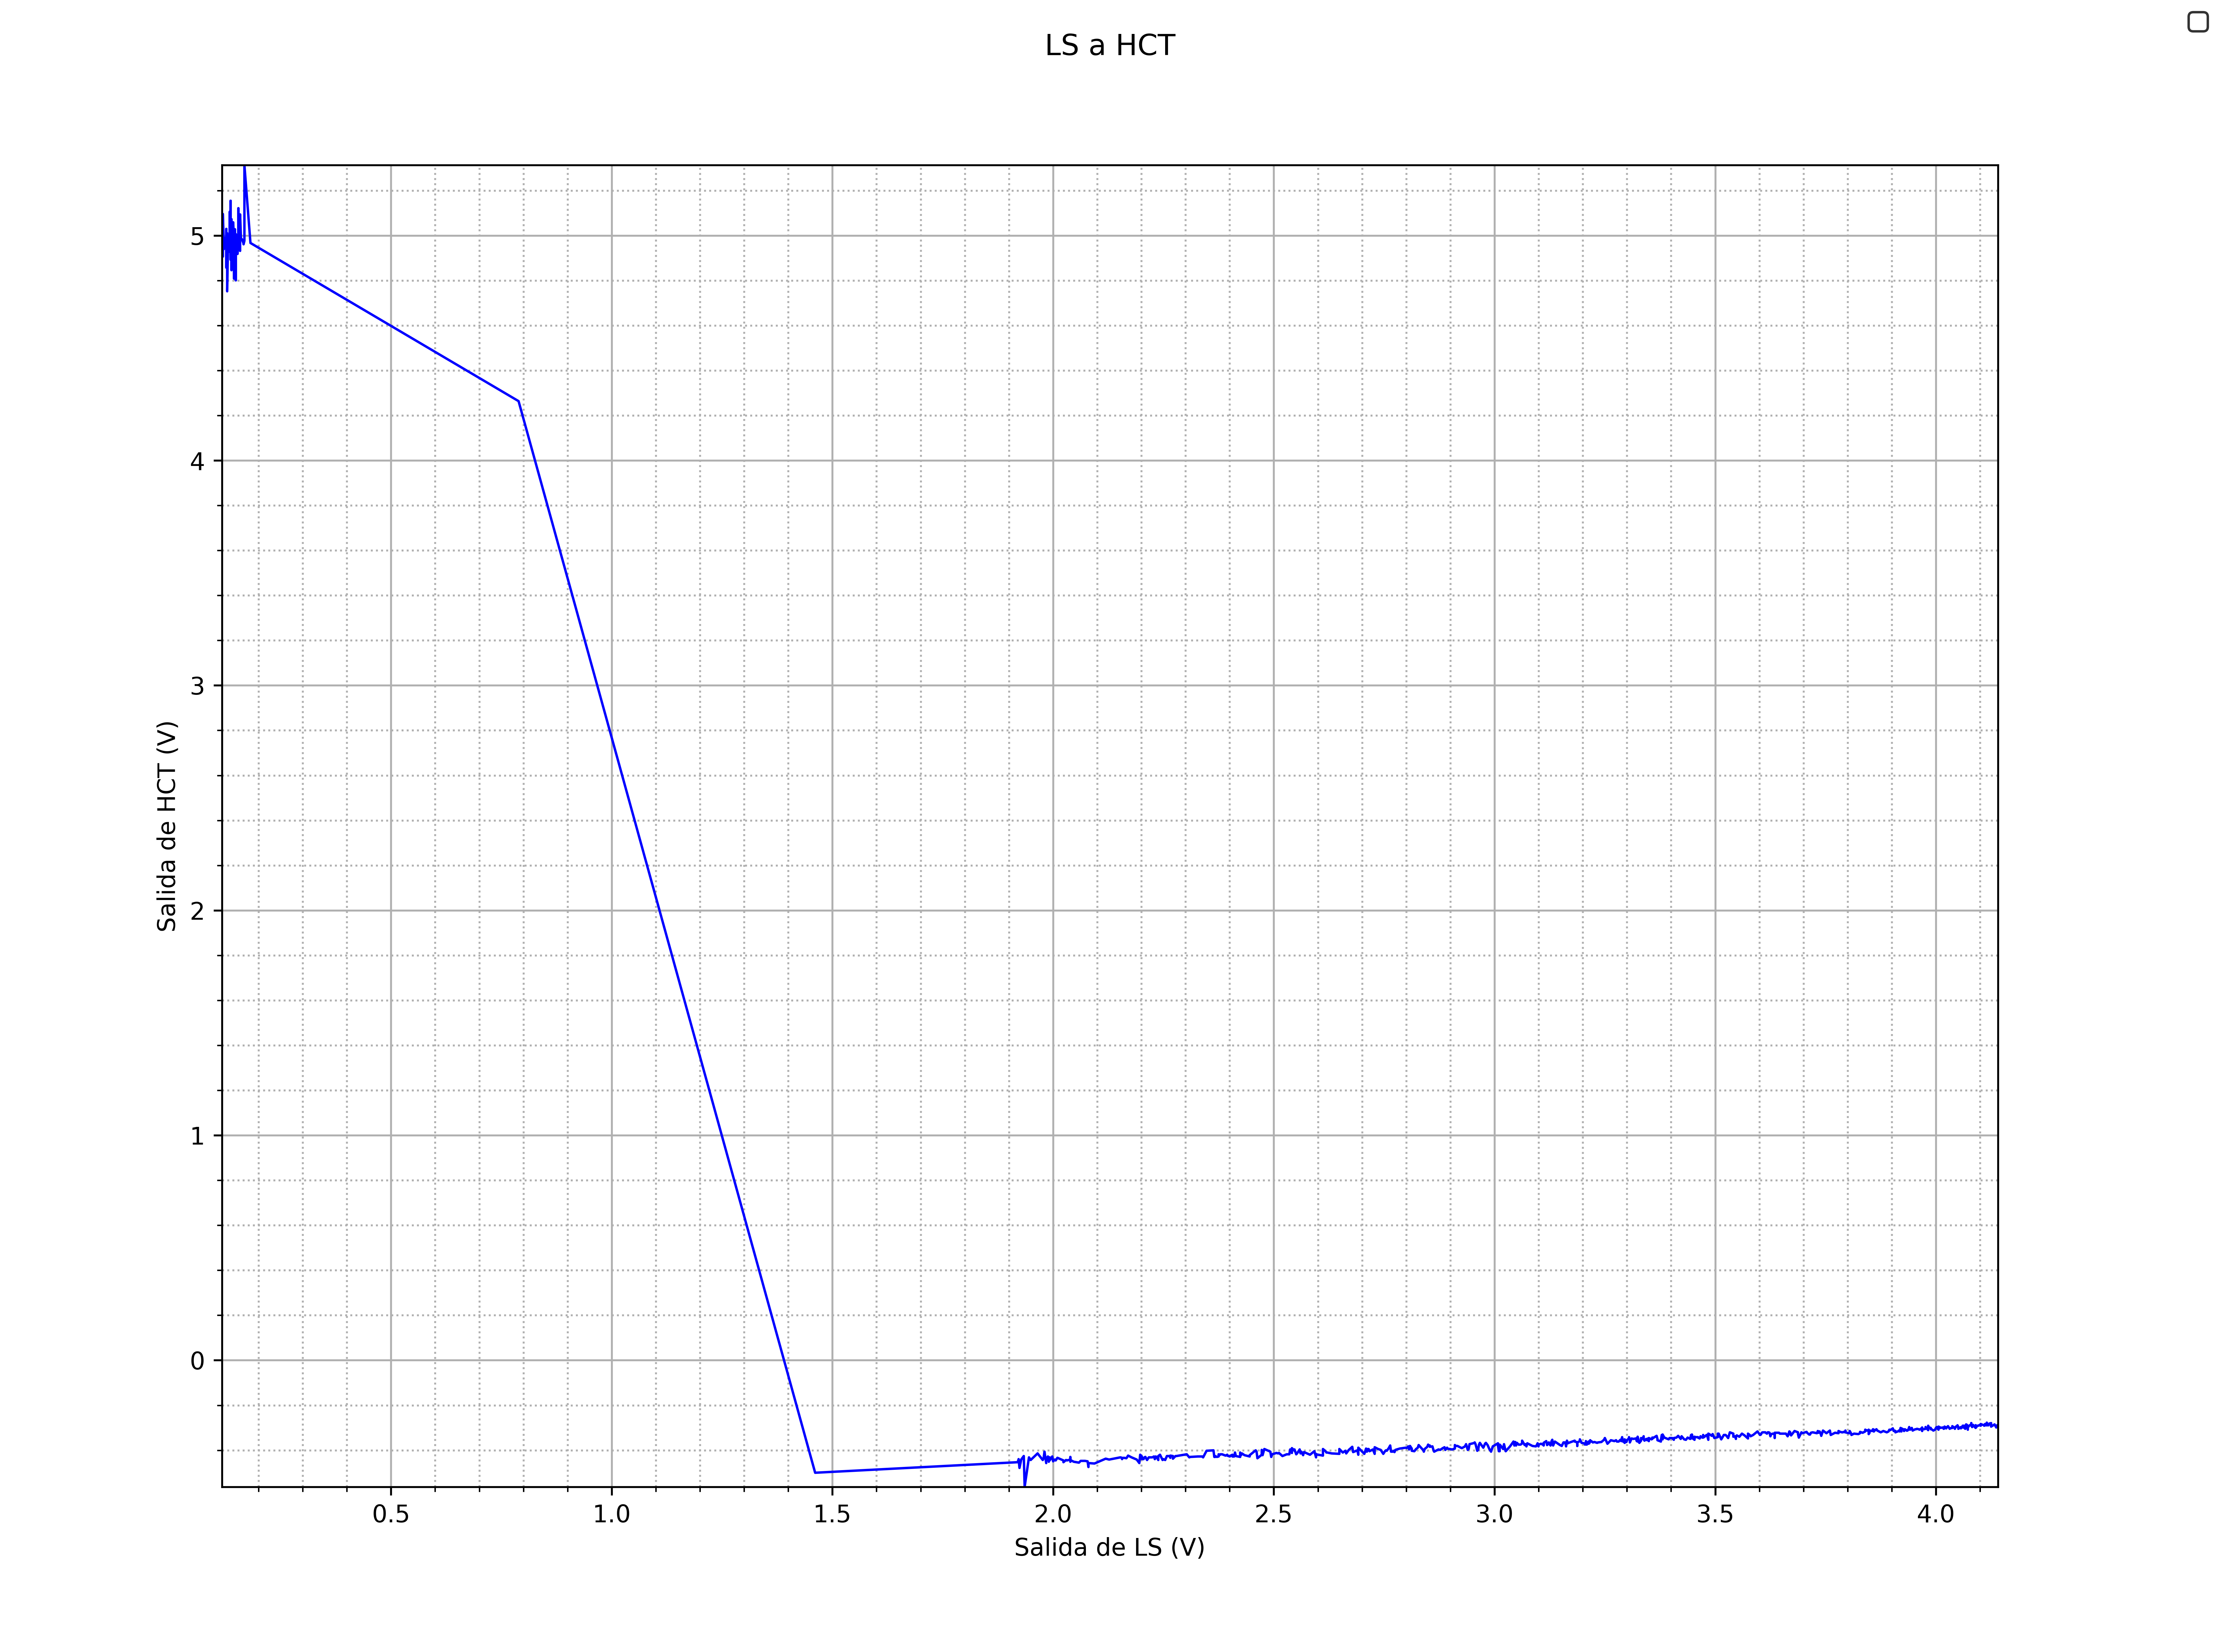
\includegraphics[width=0.5\textwidth]{../EJ2/Recursos/LS_L_v_HCT_H}
    \end{tabular}
    \caption{LS a HCT, con LS pasando de 0 a 1, y HCT de 1 a 0.}
    \label{fig:LS_L_v_HCT_H_ex5}
\end{figure}
\begin{figure}[H]
    \centering
    \begin{tabular}{c c}
        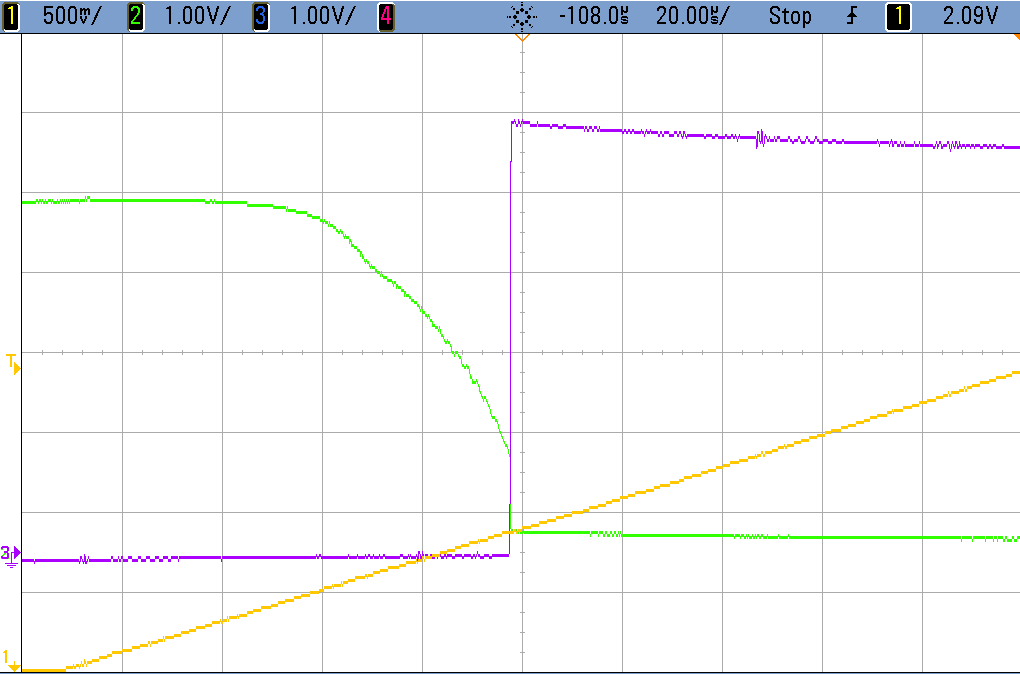
\includegraphics[width=0.5\textwidth]{../EJ2/Recursos/scope_35} &
        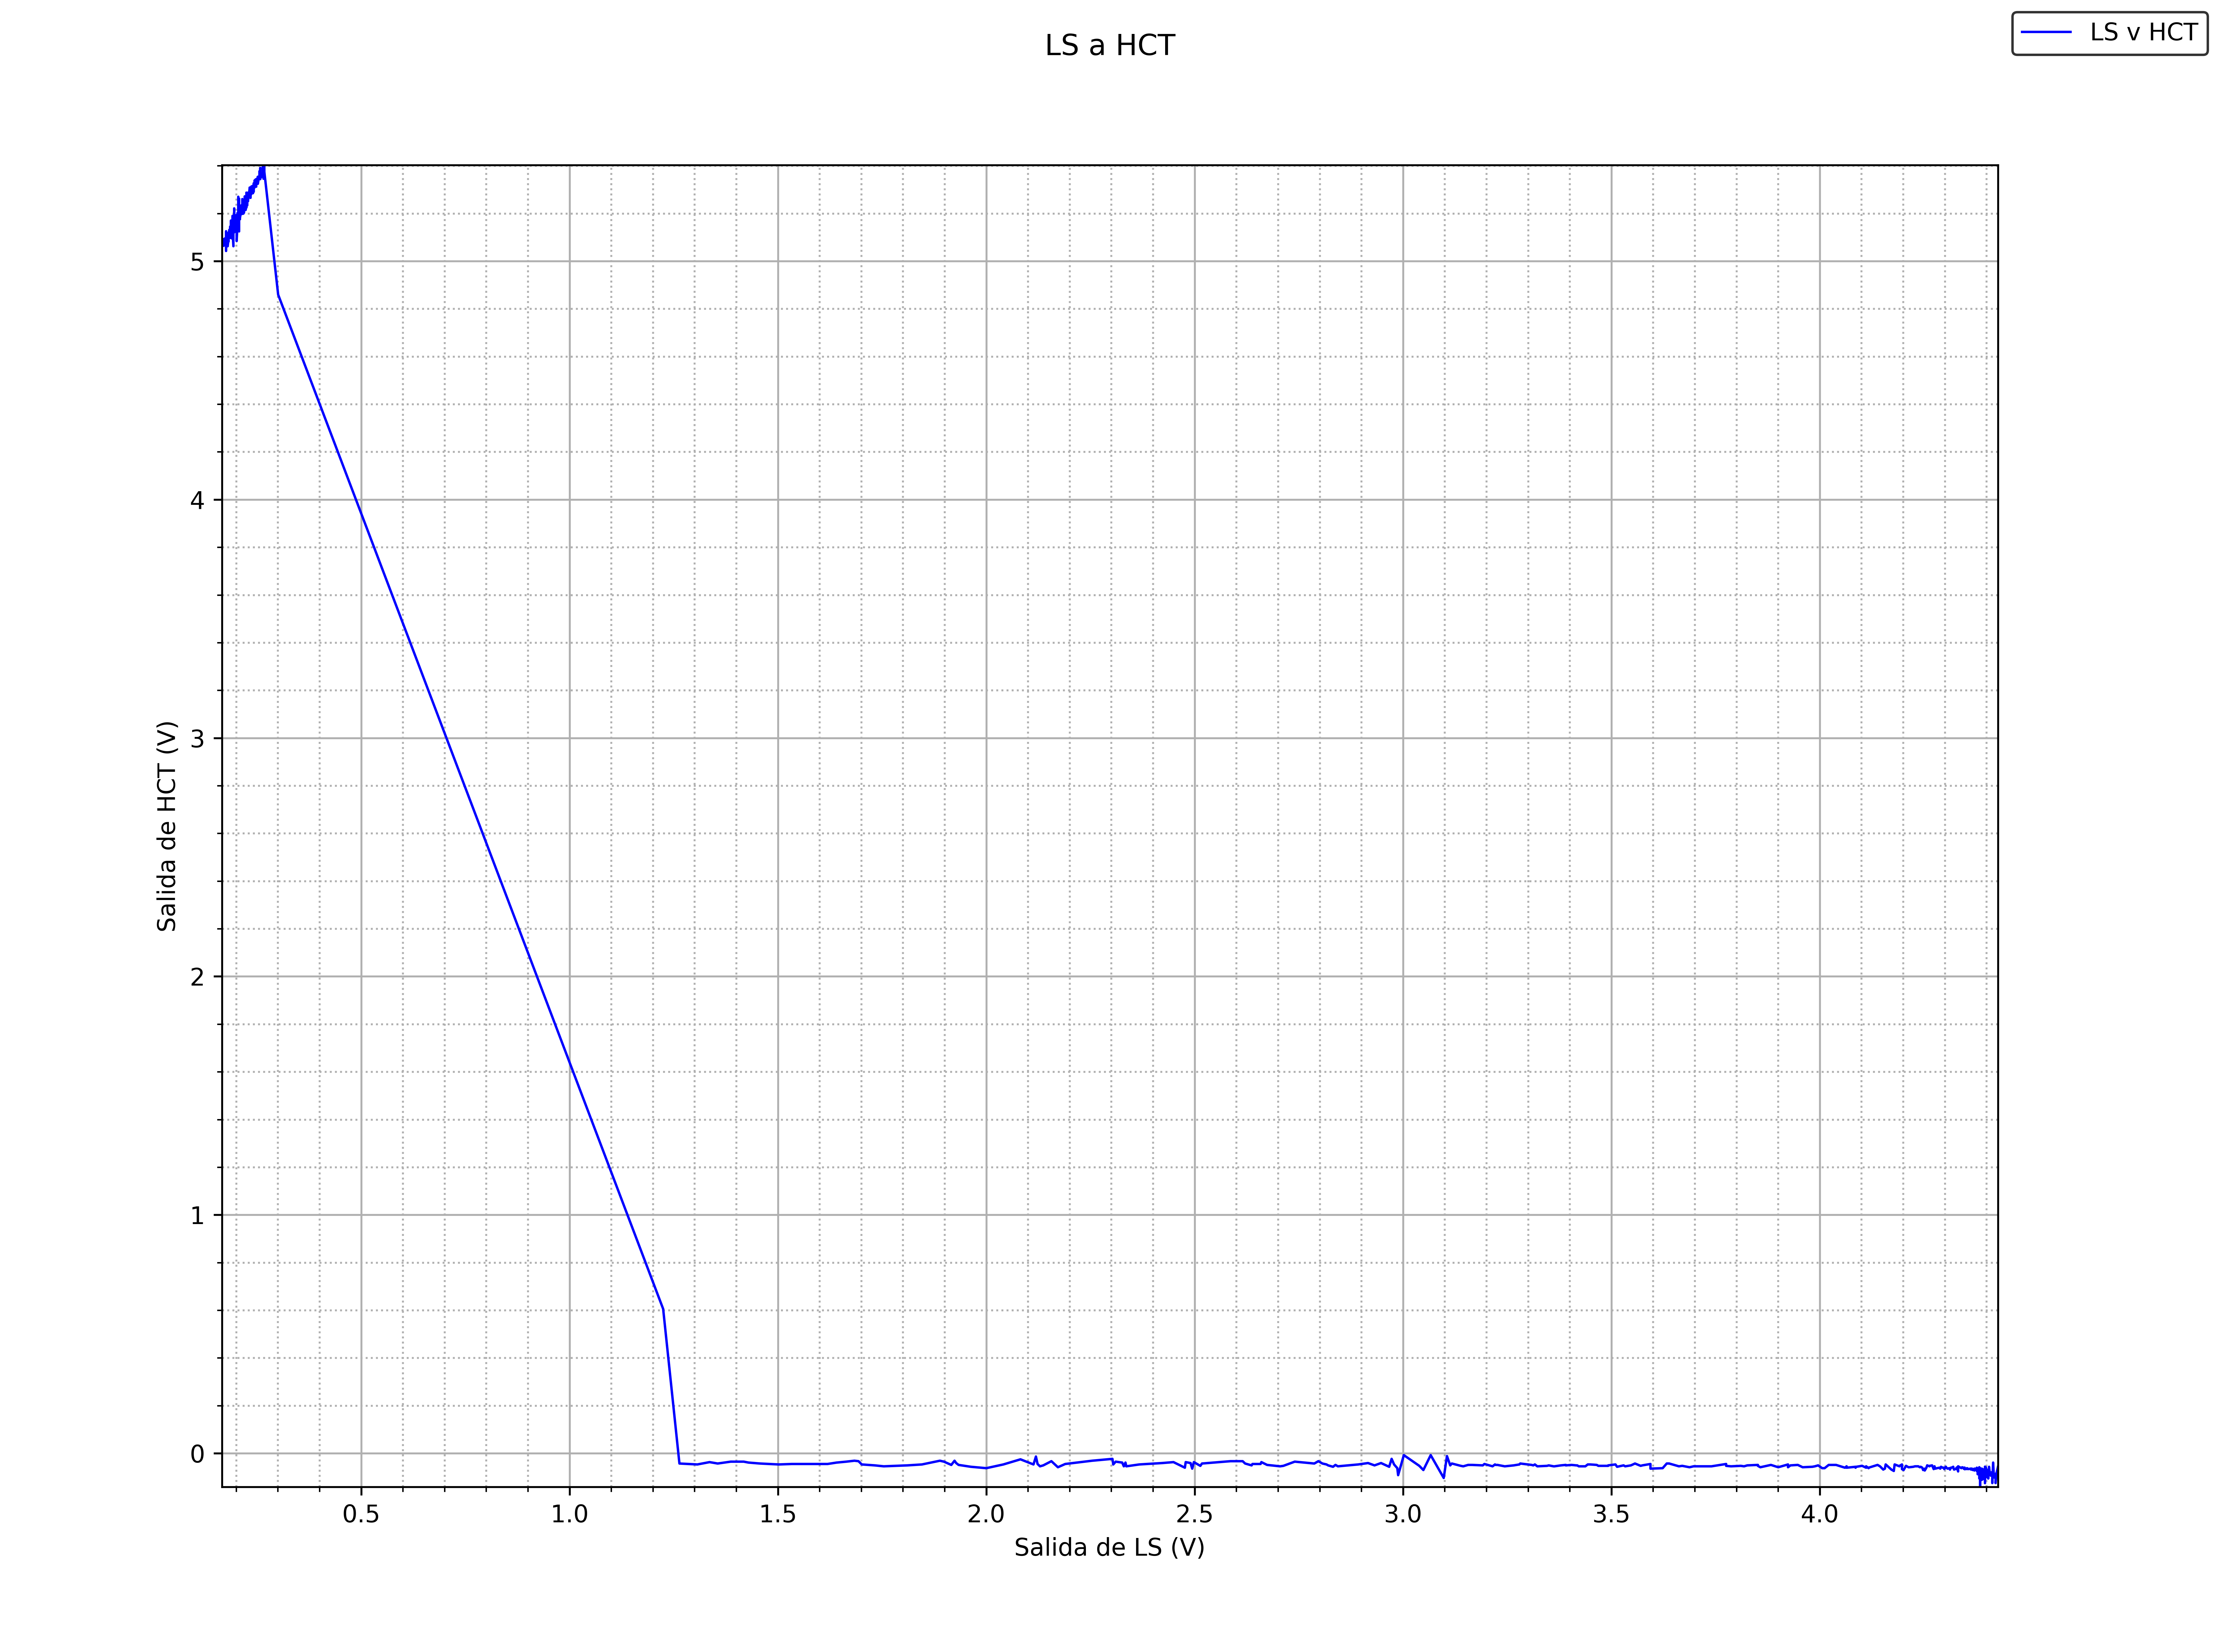
\includegraphics[width=0.5\textwidth]{../EJ2/Recursos/LS_H_v_HCT_L}
    \end{tabular}
    \caption{LS a HCT, con LS pasando de 1 a 0, y HCT de 0 a 1.}
    \label{fig:LS_H_v_HCT_L_ex5}
\end{figure}

Efectivamente lo esperado es lo que se obtiene en las mediciones, donde se puede apreciar una zona de indeterminación y oscilación en las transiciones de la configuración 
LS a HC.
Estos fenómenos no se observan luego en la configuración LS a HCT, en concordancia con lo estudiado de las hojas de datos, donde se aseguraba su compatibilidad.



\subsection{Conclusión}
A modo de cierre, se llega a la conclusión que la compatibilidad de tecnologías es un factor a tener en cuenta a la hora de realizar un diseño con compuertas lógicas de 
más de un tipo, si se quieren evitar estados indeterminados o glitches producto de transiciones con oscilaciones, causadas por incompatibilidades.
Se debe prestar especial atención al paso de tecnologías TTL a CMOS, y de ser necesario implementarlo, debe hacerse uso de compuertas CMOS especialmente diseñadas para 
esa aplicación, como lo son las de tipo HCT.
>>>>>>> master
